\documentclass[14pt,a4paper]{extarticle}
\usepackage[czech]{babel}
\usepackage[utf8]{inputenc}
\usepackage[T1]{fontenc}
\usepackage[nopatch=item]{microtype}
\usepackage{graphicx}
\usepackage{amsmath}
\usepackage{amsthm}
\usepackage{amssymb}
\usepackage{subfiles}
\usepackage{hyperref}
\usepackage{geometry}
\usepackage{mathtools}
\usepackage{algpseudocode}
\usepackage{algorithm}
\usepackage{physics}
\usepackage{dsfont}
\usepackage{bm}
\usepackage{bbm}
\usepackage{float}
\usepackage{enumitem}
\usepackage{graphicx}
\usepackage{multirow}
\usepackage{tikz}
\usepackage{tikz-cd}
\usepackage{pgfplots}
\usepackage{lmodern}
\usepackage{import}
\usepackage{fancyhdr}
\usepackage{parskip}
\usepackage{authblk}
\usepackage{listofitems}

\usepackage{mystyle}

\begin{document}
\maketitle

% % Author: Izaak Neutelings (September 2021)
% \vspace*{2cm}
% \begin{center}
%     \begin{tikzpicture}[x=2.5cm,y=1.6cm]
%         \readlist\Nnod{4,5,5,5,3}
%         \readlist\Nstr{n,m,m,m,k}
%         \readlist\Cstr{\strut x,a^{(\prev)},a^{(\prev)},a^{(\prev)},y}
%         \def\yshift{0.5}
%         \message{^^J  Layer}
%         \foreachitem \N \in \Nnod{
%             \def\lay{\Ncnt}
%             \pgfmathsetmacro\prev{int(\Ncnt-1)}
%             \message{\lay,}
%             \foreach \i [evaluate={\c=int(\i==\N); \y=\N/2-\i-\c*\yshift;
%                         \index=(\i<\N?int(\i):"\Nstr[\lay]");
%                         \x=\lay; \n=\nstyle;}] in {1,...,\N}{
%                     \node[node \n] (N\lay-\i) at (\x,\y) {$\Cstr[\lay]_{\index}$};
%                     \ifnum\lay>1
%                         \foreach \j in {1,...,\Nnod[\prev]}{
%                                 \draw[connect,white,line width=1.2] (N\prev-\j) -- (N\lay-\i);
%                                 \draw[connect] (N\prev-\j) -- (N\lay-\i);
%                             }
%                     \fi
%                 }
%             \path (N\lay-\N) --++ (0,1+\yshift) node[midway,scale=1.5] {$\vdots$};
%         }
%     \end{tikzpicture}
% \end{center}

\newpage
\tableofcontents

\documentclass[../main.tex]{subfiles}
\begin{document}
\section{Úvod}

Ahoj,

tento text jsem sepsal v rámci přípravy na zkoušku z BI-ML1. Jedná se o přehled klíčových konceptů, které mi osobně přišly důležité nebo zajímavé. Text byl zamýšlen jen pro osobní použití, ale možná ti také pomůže. K materiálu přistupuj prosím opatrně. Pro hlubší porozumění doporučuji následující učebnice:
\begin{itemize}
    \item Murphy K. P.: Probabilistic Machine Learning: An Introduction.
    \item Bishop Ch. M.: Pattern Recognition and Machine Learning.
    \item Hastie T., Tibshirani R., Friedman J.: The Elements of Statistical Learning.
\end{itemize}

Přeji příjemné studium!

\begin{flushright}
    TCH
\end{flushright}

\end{document}

\section{Rozhodovací stromy}

Na vstup předpokládáme tabulku s~$N$ záznamy a $p$ příznaky $X_0, \ldots, X_{p-1}$. Cílem je vytvořit rozhodovací strom který přiřadí co nejvíce vstupům co nejpřesnější hodnoty $Y$. Exhaustive search takového optimálního stromu je NP-úplný problém, existují však algoritmy nabízející kompromis. Pro klasifikaci ID3 a pro regresi CART nabízejí suboptimální ale dosažitelné řešení.

\subsection{Algoritmus ID3}

Algoritmus ID3 je hladový algoritmus pro konstrukci rozhodovacího stromu. V~každém vrcholu hledá podle zadaného kritéria nejlepší test (rozhodovací pravidlo) nepoužitých příznaků, které nejlépe rozdělí data na dvě podmnožiny, které maximalizují vybrané kritérium.

Algoritmus začíná s~celým datasetem a rekurzivně se zanořuje do synů, dokud nenastane zastavovací kritérium (typicky max hloubka, malý počet záznamů v~listech, ...).

\subsection{Kritéria pro větvení}

\subsubsection{Míra neuspořádanosti}

Na binární množině kde $p_0$ a $p_1$ označují poměry 0 a 1, definujeme míru neuspořádanosti jako funkci $p_0$ splňující:
\begin{enumerate}
    \item nezápornost na $[0, 1]$,
    \item nulovost pro $p_0 = 1$ nebo $p_0 = 0$,
    \item maximum nabývá v~$p_0 = \frac{1}{2}$,
    \item je rostoucí na $\left[0, \frac{1}{2}\right]$ a klesající na $\left[\frac{1}{2}, 1\right]$
\end{enumerate}

\subsubsection{Entropie}

Definici míry neuspořádanosti například splňuje entropie.
\[
    H(\D) = -p_0 \log p_0 - (1-p_0) \log (1-p_0)
\]

Entropii lze definovat i pro nebinární hodnoty.
\[
    H(\D) = - \sum_{i=0}^{k-1} p_i \log p_i
\]

Entropie (pojem z~teorie informace) používá dvojkový logaritmus a pracuje s~jednotkou bit (Claude Shannon).

\subsubsection{Gini index}

Místo entropie lze použít gini index (gini impurity), které má podobné vlastnosti.
\[
    GI(\D) = \sum_{i=0}^{k-1} p_i (1 - p_i)
\]

\subsubsection{Informační zisk}

Příznak pro rozdělení se volí podle informačního zisku
\[
    IG(\D) = H(\D) - t_0 H(\D_0) - t_1 H(\D_1)
\]

kde $\D_0, \D_1$ jsou příslušné podmnožiny $\D$ a $t_0, t_1$ poměry počtu 0 a 1 v~$Y$.

\subsection{Použití pro klasifikaci a regresi}

\subsubsection{Klasifikace}

V~případě klasifikace strom rozhoduje většinovým hlasováním v~příslušném listu, do kterého záznam přísluší. Poměr výsledného prvku v~listu určuje jistotu modelu při takové volbě.

\subsubsection{Regrese}

U~regrese se rozhoduje podle průměru v~příslušném listu.

Konstrukce stromu v~regresní úloze probíhá podobně jako v~klasifikační. Místo minimalizace míry neuspořádanosti, algoritmus dělí data tak, aby byly hodnoty v~listech co nejblíže ke střední hodnotě.

Pro odhad odchylky od střední hodnoty se používá MSE (mean squared error), případně MAE (mean absolute error).

\begin{equation*}
    \begin{aligned}[t]
        \MSE(\mathbf{Y}) = \frac{1}{N} \sum_{i=0}^{N-1} (Y_i - \bar{Y})^2
    \end{aligned}
    \qquad
    \begin{aligned}[t]
        \MAE(\mathbf{Y}) = \frac{1}{N} \sum_{i=0}^{N-1} |Y_i - \bar{Y}|
    \end{aligned}
\end{equation*}

Hladovému algoritmu konstrukce stromu, ve kterém se minimalizuje MSE, se říká CART (classification and regression trees).

Jako alternativu informačního zisku (ID3), používá CART
\begin{equation*}
    \MSE(\D) - t_0 \MSE(\D_0) - t_1 \MSE(\D_1)
\end{equation*}

\subsection{Hyperparametry}

Rozhodovací stromy mají často nízký bias a vysokou varianci. Jako hyperparametry rozhodovacího stromu můžeme volit různá ukončovací pravidla, kterými zamezit přeučení.
\begin{enumerate}
    \item dělící kritérium
          \begin{enumerate}
              \item gini, entropy (klasifikace)
              \item squared error, absolute error (u~regrese)
          \end{enumerate}
    \item max hloubka, od které algoritmus už dále nedělí
    \item minimální počet dat v~množině před, resp. po, dělení
    \item minimální nutná hodnota informačního zisku
\end{enumerate}

\subsection{Shrnutí}

Rozhodovací stromy jsou nenáročné na přípravu, jsou dobře interpretovatelné, jednoduché a rychlé. Jsou však nerobustní a je snadné je přeučit.

\section{Metoda nejbližších sousedů kNN}

Metoda nejbližších sousedů je model supervizovaného učení, které predikuje na základě nejbližších záznamů ve vícedimenzionálním prostoru trénovacích dat.

\subsection{Hyperparametry}

\subsubsection{Počet sousedů k}

Číslo $k$ určuje počet nejbližších sousedů, ze kterých model počítá predikci. Vyšší hodnota zabraňuje přeučení.

\subsubsection{Vzdálenost (metrika)} \label{sec:metrika}

Metrika na množině $\calX$ je funkce $d: \calX \times \calX \longrightarrow [0, +\infty)$ taková, že pro každé $x, y, z \in \calX$ platí
\begin{enumerate}
    \item pozitivní definitnost: $d(x, y) \ge 0 \land d(x, y) = 0$ právě tehdy když $x = y$
    \item symetrie: $d(x,y) = d(y,x)$
    \item trojúhelníková nerovnost: $d(x, y) + d(y, z) \ge d(x, z)$
\end{enumerate}

Častými metrikami jsou Minkowského k-metriky ($L_k$ vzdálenosti)
\[
    \|\x - \y\|_k = d_k(\x, \y)_k = \sqrt[k]{\sum_{i=0}^{p-1} |x_i - y_i|^k}
\]

Speciálně pro $k=1$ dostáváme Manhattanskou vzdálenost
\[
    d_1(\x, \y) = \sum_{i=0}^{p-1} |x_i - y_i|
\]

Pro $k=2$ Eukleidovskou vzdálenost
\[
    d_2(\x, \y) = \sqrt{\sum_{i=0}^{p-1} (x_i - y_i)^2}
\]

A~pro $k=+\infty$ Chebyshevovu vzdálenost
\[
    d_{\infty}(\x, \y) = \max_i |x_i - y_i|
\]

Příklad dalších často používaných metrik je Levenshteinova editační vzdálenost dvou řetězců nebo kosinová vzdálenost dvou vektorů podle úhlu (pouze pozitivně semidefinitní), které svírají
\[
    d(\x, \y) = \frac{\x \cdot \y}{\|\x\|_2 \|\y\|_2}
\]

Existují i sofistikovanější metriky jako je například Jaccardova pro množiny nebo Haversinova pro vzdálenost dvou bodů na sféře.

\subsubsection{Váha sousedů}

U~regresních úloh může být váha sousedů uniformní (každý z~$k$ sousedů má stejný vliv na výsledek predikce)
\[
    \hat{y} = \frac{1}{k} \sum_{i=0}^{k-1} y_k
\]
nebo může být vážený podle vzdálenosti (bližší soused je vlivnější)
\begin{equation*}
    \begin{aligned}[t]
        \hat{y} = \frac{\sum_{i=0}^{k-1} w_i y_k}{\sum_{i=0}^{k-1} w_i}
    \end{aligned}
    \quad \text{kde} \quad
    \begin{aligned}[t]
        w_i = \frac{1}{d(\x_i, \bm{n}_i)}
    \end{aligned}
\end{equation*}

\subsection{Použití pro klasifikaci a regresi}

Pro trénovací data $\X \in \R^{N, p}$ s~vysvětlovanou proměnou $Y \in \R^N$ predikujeme hodnotu vysvětlované proměnné pro datový bod $\x \in \R^p$ hlasováním (klasifikace), případně průměrem (regrese), $k$ nejbližších sousedů.

Model kNN má tak velmi levné ``trénování", kdy pouze ukládá trénovací množinu do paměti. Predikce je ovšem výpočetně náročnější.

\subsection{Normalizace dat}

Kvůli rozdílným rozsahům příznaků mají rozsahy hodnot v~původních datech nerovnoměrný příspěvek na vzdálenost. Tento problém se dá řešit normalizací do intervalu $[0,1]$, případně $[-1, 1]$, nebo standardizací.

\begin{equation*}
    \text{normalizace: }
    \begin{aligned}[t]
        x_i \leftarrow \frac{x_i - \text{min}_x}{\text{max}_x - \text{min}_x}
    \end{aligned}
    \quad\quad
    \text{standardizace: }
    \begin{aligned}[t]
        x_i \leftarrow \frac{x_i - \bar{x}}{\sqrt{s_x^2}}
    \end{aligned}
\end{equation*}

Normalizace není vždy přímočará. Někdy se vyplatí normalizovat jen některé příznaky, nebo do různě velkých rozsahů, čímž se přiřadí umělá váha.

\subsection{Prokletí dimenzionality}

Metodě kNN neprospívá vysoká dimenzionalita. S~vyšší dimenzionalitou rostou vzdálenosti všech bodů a může se stát, že v~případě řídkých dat je okolí, co do vzdálenosti, prázdné nebo nereprezentativní (rozdíl vzdálenosti vzdálených a blízkých bodů se zmenšuje).

Nominální data se předzpracovávají pomocí OHE, což kvůli těmto problémům není ideální. Problém představuje také přítomnost méně relevantní příznaků, protože se model chová ke všem rozměrům stejně.

Pro rostoucí počet dimenzí významně roste potřebný počet prvků pro zaplnění prostoru a reprezentativní predikce.

\section{Lineární regrese}

V~modelu lineární regrese předpokládáme lineární závislost vysvětlované proměnné na hodnotách příznaků.

\subsection{Model}

Pro data s~hodnotami příznaků $X_1, \ldots, X_p$ a hodnotou vysvětlované proměnné $Y$ předpokládáme lineární model
\begin{equation*}
    Y = w_0 + w_1 X_1 + \ldots + w_p X_p + \varepsilon
\end{equation*}

kde $w_i$ jsou neznámé koeficienty a $\varepsilon$ představuje chybu nebo nekonzistenci výsledné hodnoty $Y$, kterou model nezachycuje a pro kterou platí $\E \varepsilon = 0$.

V~bodě $(x_1, \ldots, x_p)^T$ tohoto modelu platí vztah \[ Y = w_0 + w_1 x_1 + \ldots + w_p x_p + \varepsilon = \we^T \x + \varepsilon \] kde zavádíme následující vektorovou notaci pro vstup $\x$ a vektor vah $\we$
\begin{align*}
    \x  & = (1, x_1, \ldots, x_p)^T   \\
    \we & = (w_0, w_1, \ldots, w_p)^T
\end{align*}

\subsection{Predikce}

S~odhadnutými váhami $\hat{\we}$ predikujeme vztahem
\[\hat{Y} = \hat{\we}^T\x = \hat{w_0} + \hat{w_1} x_1 + \ldots + \hat{w_p} x_p\]

Pro skutečnou hodnoty $Y = \we^T \x + \varepsilon$ platí z~předpokladu $\E \varepsilon = 0$ \[\E Y = \E \we^T \x + \E \varepsilon = \we^T \x\]

$\hat{Y}$ je tedy bodovým odhadem $EY$ v~bodě $\x$.

\subsection{Metoda nejmenších čtverců}

Metoda nejmenších čtverců nalézá hodnotu $\hat{\we}$ odhadu $\we$ minimalizací následující kvadratické ztrátové funkce: \[L(Y, \hat{Y}) = (Y - \hat{Y})^2\]

Pro trénovací množinou $(\x_i, Y_i), i = 1, \ldots, N$ minimalizujeme reziduální součet čtverců
\[ \RSS(\we) = \sum_{i = 1}^{N} L(Y_i, \hat{Y}_i) = \sum_{i = 1}^{N} (Y_i - \we^T \x_i)^2 \]

\subsubsection{Maticový zápis trénovací množiny}

Zavádíme náhodné vektory $\Y = (Y_1, \ldots, Y_N)^T, \bm{\varepsilon} = (\varepsilon_1, \ldots, \varepsilon_N)$ a body $\x_1, \ldots, \x_N$ zapisujeme do řádků matice
\begin{equation*}
    \X =
    \begin{pmatrix}
        \x_1^T \\
        \vdots \\
        \x_N^T
    \end{pmatrix}
    =
    \begin{pmatrix}
        1      & x_{1,1} & \cdots & x_{1,p} \\
        \vdots & \vdots  & \ddots & \vdots  \\
        1      & x_{N,1} & \cdots & x_{N,p} \\
    \end{pmatrix}
    \in \R^{N, p+1}
\end{equation*}

Při tomto značení platí rovnice $\Y = \X\we + \bm{\varepsilon}$ kde $\E \bm{\varepsilon} = \mathbf{0}$.

\subsubsection{Minimalizace RSS}

\[ \RSS(\we) = \sum_{i=1}^{N} (Y_i - \we^T \x_i)^2  = \| \Y - \X \we \|^2 \]

Začneme nalezením gradientu této funkce
\begin{align*}
    \pdv{\RSS(\we)}{w_j}
     & = \sum_{i=1}^{N} 2 (Y_i - \we^T \x_i) (-x_{i, j}) \\
    \nabla \RSS(\we)
     & = \sum_{i=1}^{N} 2 (Y_i - \we^T \x_i) (-\x_i)     \\
     & = -2 \X^T (\Y - \X\we)
\end{align*}

Položením $\nabla \RSS(\we) = \mathbf{0}$ obdržíme normální rovnici
\[ \X^T \Y - \X^T \X\we = \mathbf{0}. \]

Předpokládáme-li, že $\X^T\X$ je regulární, pak lze $\we$ odhadnout následovně
\[ \wh_{\text{OLS}} = (\X^T \X)^{-1} \X^T \Y \]

V~případě regulární matice $\X^T\X$ je $\wh_{\text{OLS}}$ jediným kritickým bodem. Z~geometrické interpretace, kterou dosáhneme stejného výsledku, bude plynout, že se jedná o~globální minimum $\RSS(\we)$.

Predikce $\hat{Y}$ v~bodě $\x$ je $\hat{Y} = \wh_{\text{OLS}}^T \x$.

\subsubsection{Geometrická interpretace}

Minimalizace $\RSS(\we) = \| \Y - \X \we \|^2$ je problém ekvivalentní minimalizaci ${\| \Y - \X \we \|}$. Hledáme tedy $\we \in \R^{p+1}$ takové, že vektory $\Y$ a $\X\we$ jsou si v~prostoru $\R^{N}$ co nejblíže.

$\X\we$ je lineární kombinací sloupců $\X$:
\[ \X\we = \sum_{i=0}^{p} \we_i \X_{:,i} \in \langle \X_{:,0}, \X_{:,1}, \ldots, \X_{:,p} \rangle = \bm{P} \]

Hledaný bod $\X\we$ je proto nejblíže k~bodu $\Y$, právě pokud je vektor $\Y - \X\we$ ortogonální na podprostor $\bm{P}$:
\[ \X_{:,i}^T(\Y - \X\we) = 0 \text{ pro všechna } i = 0, 1, \ldots, p \]
Což po přepsání do maticového tvaru dá opět normální rovnici

\[ \X^T(\Y - \X\we) = \X^T\Y - \X^T\X\we = \bm{0} \]

Z~úvah také navíc plyne, že každé $\wh$, které splňuje normální rovnici, $\RSS(\we)$ minimalizuje (jedná se o~globální minimum).

\subsection{Regularita versus lineární nezávislost sloupců matice X}

Pro libovolné $\bm{s} \in \R^{p+1}$ platí následující posloupnost implikací:
\[
    \X^T\X\bm{s} = \mathbf{0}
    \Rightarrow \bm{s}^T\X^T\X\bm{s} = \|\X\bm{s}\|^2 = 0
    \Rightarrow \X\bm{s} = \bm{0}
    \Rightarrow \X^T\X\bm{s} = \mathbf{0}
\]

Z~toho vyplývá, že $\X^T\X$ je regulární právě tehdy, když $\X\bm{s} = \bm{0}$ pouze pro $\bm{s} = \bm{0}$, což platí právě tehdy, když jsou sloupce matice $\X$ lineárně nezávislé. To zřejmě nemusí vždy platit: např. když $N < p+1$ nebo pokud je nějaký příznak lineární kombinací ostatních.

Normální rovnice má v~případě regulární $\X^T \X$ právě jedno řešení.
\[ \wh_{\text{OLS}} = (\X^T \X)^{-1} \X^T \Y \]
V~opačném případě má jich má nekonečně mnoho.

\subsection{Problém kolinearity}

Pokud je nějaký příznak ``skoro'' lineární kombinací ostatních příznaků, pak můžeme narazit na problém kolinearity. V~případě silně korelovaného příznaku je příslušná proměnná do jisté míry zbytečná, protože ve svém rozměru (dimenzi) nepřidává žádnou informaci navíc a zároveň může mít ve výsledném vektoru $\wh_{\text{OLS}}$ vysoký koeficient. Jako příklad lze uvést 3-dimenzionální prostor ($X_1, X_2, Y$) ve kterém řešení degeneruje do skoro-přímky, kterou lze protnou rovinou více způsoby.

\subsubsection{Důsledky kolinearity}

Ve výsledku kolinearita způsobuje vysoký rozptyl $\wh_{\text{OLS}}$, který je tak velmi citlivý na data. Pro různé realizace stejného náhodného výběru se řešení normální rovnice může značně lišit. Vysoký rozptyl se následovně přenáší na predikce, které jsou pak méně spolehlivé.

\subsubsection{Řešení problému kolinearity}

Řešením by bylo odstranit příznaky, které kolinearity způsobují. To však není vždy jednoduché. S~vyšším počtem příznaků je velmi obtížné takové sloupce identifikovat. Také se může stát, že kolinearita je mezi velkým počtem příznaků, které jsou dohromady klíčové pro správnou predikci. V~takovém případě není ideální takové příznaky zahodit. Existují však metody, které dokážou počet příznaků snížit (odstraněním, případně nahrazením menším počtem) tak, aby byly sloupce LN.

Je také možné změnit funkci, kterou minimalizujeme, abychom měli stabilnější a jednoznačnější řešení. Typicky se přidává regulační člen, který problémy kolinearity může zmírnit (hřebenová regrese v~sekci \ref{sec:ridge} nebo lasso v~sekci \ref{sec:lasso}).

\subsection{Shrnutí}

Lineární regrese je rezistentní vůči problémům spojené s~vysokou dimenzí dat. Problém nastává, když je dat méně než příznaků nebo když jsou příznaky silně korelované.

\section{Hřebenová regrese} \label{sec:ridge}

Hřebenová nebo také $L_2$ regularizace, stejně jako lineární regrese, předpokládá lineární model $Y = \we^T \x + \varepsilon$. Nicméně navíc řeší problém kolinearity tím, že penalizuje vysoké hodnoty koeficientů $\we$ vyjma interceptu.

\subsection{Regularizovaný reziduální součet čtverců}

Hřebenová regrese tedy minimalizuje následují reziduální součet čtverců
\[ \RSS_\lambda(\we) = \| \Y - \X \we \|^2 + \lambda \sum_{i=1}^{p} w_i^2 \]
s~regulačním členem $\lambda \ge 0$.

Pro $\lambda = 0$ dostáváme klasickou neregularizovanou lineární regresi. Intercept se nepenalizuje, protože ten jen zajišťuje $\E \varepsilon = 0$.

\subsection{Minimalizace regularizovaného RSS}

Pro účely hřebenové regrese zavedeme
\[\mathbf{}
    \I' =
    \begin{pmatrix}
        0      & 0      & \cdots & 0      \\
        0      & 1      & \cdots & 0      \\
        \vdots & \vdots & \ddots & \vdots \\
        0      & 0      & \cdots & 1
    \end{pmatrix}
    \in \R^{p+1, p+1}
\]

Regularizovaný $\RSS_\lambda$ lze vyjádřit Jako
\begin{align*}
    \RSS_\lambda(\we)
     & = \| \Y - \X \we \|^2 + \lambda \sum_{i=1}^{p} w_i^2  \\
     & = \| \Y - \X \we \|^2 + \lambda \we^T \I' \we
\end{align*}

Nalezneme parciální derivaci a následně gradient
\begin{align*}
    \pdv{\RSS(\we)}{w_j}
     & = \sum_{i=1}^{N} 2 (Y_i - \we^T \x_i) (-x_{i, j}) + 2 \lambda w_j         \\
    \nabla \RSS(\we)
     & = \sum_{i=1}^{N} 2 (Y_i - \we^T \x_i) (-\x_i) + 2 \lambda \I' \we \\
     & = -2 \X^T (\Y - \X\we) + 2 \lambda \I' \we
\end{align*}

A~položením rovno nule obdržíme ekvivalent normální rovnice

\begin{align*}
    \X^T\Y - \X^T\X\we - \lambda \I' \we & = 0 \\
    \X^T\Y - (\X^T\X + \lambda \I') \we  & = 0
\end{align*}

Hessova matice zde vychází
\[
    \textbf{H}_{\RSS_\lambda}(\we) = 2(\X^T\X - \lambda \I')
\]

Pro libovolné $\bm{s} \in \R^{p+1}, \bm{s} \ne \bm{0}, \lambda > 0$ platí
\begin{align*}
    \bm{s}^T(\X^T\X + \lambda \I')\bm{s}
     & = \bm{s}^T \X^T\X \bm{s} + \lambda \bm{s}^T \I' \bm{s} \\
     & = \| \X \bm{s} \|^2 + \lambda \sum_{i=1}^{p} s_i^2 > 0,
\end{align*}

Matice $\X^T\X + \lambda \I'$ je tedy vždy pozitivně definitní a regulární a řešení normální rovnice pro regulované $\RSS_\lambda$ je jednoznačné.
\[\wh_\lambda = (\X^T\X + \lambda \I')^{-1} \X^T\Y\]
Predikce modelu je $\hat{Y} = \wh_\lambda^T\x$.

\subsection{Modely bázových funkcí}

Model lineární regrese, případně hřebenové regrese, modeluje pouze lineární funkci. Množinu příznaků lze však rozšířit jejími transformovanými variantami.

\subsubsection{Bázové funkce}

Pro $M \in \mathbb{N}$ zvolme $M$ funkcí $\varphi_1, \ldots, \varphi_M$ z~$\R^{p}$ do $\R$ reprezentující transformace. Těmto funkcím říkáme bázové funkce.

Modely bázových funkcí se od předchozích lineárních regresních modelů liší pouze tím, že místo původního $\x$ pracuje s~$\bm{\varphi}(\x)  \coloneqq (1, \varphi_1(\x), \ldots, \varphi_M(\x))^T$

\subsubsection{Volba bázových funkcí}

Časté volby bázových funkcí jsou
\begin{itemize}
    \item $\varphi(\x) = x_i$ -- původní příznaky
    \item $\varphi(\x) = x_i^2, x_i x_j$ -- mocniny, součiny (polynomiální regrese)
    \item $\varphi(\x) = \log(x_i), \sqrt{x_i}, \sin(x_i)$ -- nelineární transformace
    \item $\varphi(\x) = \mathds{1}_{A}$ -- indikátory (dělení prostoru)
\end{itemize}

\subsubsection{Model}
Model bázové funkce rozšiřuje možnosti hřebenové regrese a může jej dělat velmi mocným a sofistikovaným nástrojem.
\[\x \longrightarrow \bm{\varphi(\x)} \colon \quad Y = \we_\lambda^T\bm{\varphi(\x)} + \varepsilon\]

Postup s~transformovaným vektorem $\x' \coloneqq \bm{\varphi(\x)}$ je dál zcela analogický jako u~hřebenové regrese a predikce modelu je $\hat{Y} = \wh_\lambda^T\bm{\varphi(\x)}$.

\section{Výběr příznaků}

Často je výhodné počet příznaků před trénováním modelů snížit. Proces, který zvolí nějakou výhodnou podmnožinu příznaků, je feature selection. Tento proces spadá do části předzpracování dat, konkrétně se jedná o~podoblast redukce dimenzionality (dimension reduction).

Výběrem příznaků řešíme hned několik problémů najednou:
\begin{itemize}
    \item Zahozením nerelevantních a redundantních příznaků můžeme významně zlepšit schopnost generalizace modelu (model není zatížený šumem).
    \item Pomáhá s~prokletím dimenzionality (curse of dim.), kdy vysoká dimenze způsobuje řídkost dat a nerelevantnost sousedství.
    \item Zlepšuje interpretovatelnost modelu.
    \item Snižuje výpočetní nároky pro trénování.
\end{itemize}

\subsection{Základní metody výběru příznaků}

\subsubsection{Filtrační metody}

Filtrační metody jsou jednoduché a často nevyžadují náročné trénovaní modelů:
\begin{itemize}

    \item Vyhodit příznaky s~příliš nízkým rozptylem (jsou téměř konstantní).

    \item Vyhodit příznaky, které mají příliš chybějících hodnot.

    \item Vyhodit redundantní příznaky, které mají vysokou korelaci s~jiným příznakem (jsou v~datasetu již zastoupeny).

    \item Vyhodit příznaky, které mají s~cílovou proměnnou nízkou korelaci (je dobré v~kombinaci s~bázovými funkcemi -- samotný příznak totiž nemusí vysvětlovanou proměnnou ovlivňovat pouze lineárně).

    \item U~binárních příznaků rozdělit data na dvě populace a provést hypotézu o~rovnosti středních hodnot obou populací (dvouvýběrový t-test).

    \item Provést test nezávislosti mezi příznakem a vysvětlovanou proměnnou.

\end{itemize}

\subsubsection{Obalové metody}

Obalové metody používají pro ohodnocení příznaků pomocný model, který na příslušné kandidátní množině příznaků natrénují a pak výkon porovnají se stejným modelem natrénovaný na jiné sadě příznaků.

Pokud se jako pomocný model použije finální model, je výhodou, že se zvolí tu sadu příznaků, která dobře pracuje s~vybraným modelem. V~takovém případě však snadněji dochází k~přeučení. Vybere-li se ale jiný model, sada příznaků může být zvolena nevýhodně pro finální model.

Pokud je kandidátních množin příznaků hodně, je tato metody výpočetně náročná, proto se často používají hladové algoritmy:
\begin{itemize}

    \item Dopředný výběr (forward selection) začíná s~prázdnou množinou a postupně přidává příznak, který v~dané iteraci nejvíce zvýší výkonnost modelu.

    \item Zpětný výběr (backward selection) začíná se všemi příznaky a postupně odebírá ty, které nejméně sníží výkonnost modelu.

    \item Rekurzivní odebírání příznaků (recursive feature elimination) postupně odebírá podle vnitřního ohodnocení příznaků pomocného modelu (u~norm. lineární regrese koeficienty, u~stromu příslušný informační zisk)

\end{itemize}
Algoritmy běží dokud nemají požadovaný počet příznaků, případně mohou skončit i s~menším počtem příznaků, pokud přidávání, resp. odstranění, příznaků nesnižuje výkonnost.

\subsubsection{Vestavěné metody}

Vestavěné metody (embedded methods) provedou výběr příznaků natrénováním modelu na celých datech a pak zahodí příznaky, které se naučil vůbec nepoužívat.

U~lineární regrese se jedná o~příznaky s~koeficientem 0, u~rozhodovacího stromu ty, které se nikde nepoužily, atd.

\subsection{Lasso} \label{sec:lasso}

Nejpoužívanější vestavěnou metodou je $L_1$ regularizovaná lineární regrese, která volí množinu příznaků s~nenulovým koeficientem.

Na rozdíl od hřebenové regrese penalizuje absolutní hodnotu koeficientů. Pro $\lambda \ge 0$ minimalizuje
\[
    \RSS_\lambda^\Lasso = \sum_{i=1}^{N} (Y_i - \hat{Y}_i)^2
    + \lambda \sum_{i=1}^{p} |w_i|
\]
Pro $\lambda = 0$ se jedná o~klasickou lineární regresi. Pro $\lambda > 0$ cílí na co nejmenší koeficienty, ale nevadí mu vysoké hodnoty.

$\RSS_\lambda^\Lasso$ není diferencovatelný, proto se řešení hledá iterativní metodou:
\[
    \wh_\lambda^\Lasso = \argmin_{\we} \RSS_\lambda^\Lasso (\we)
\]
Výhoda modelu Lasso je, že $\wh_\lambda^\Lasso$ je řídké -- hodně členů je rovno nule. S~vyšší $\lambda$ jsou nuly častější.

Formální důkaz tohoto tvrzení je složitý, ale pro představu lze znázornit obrázkem.

\begin{center}
    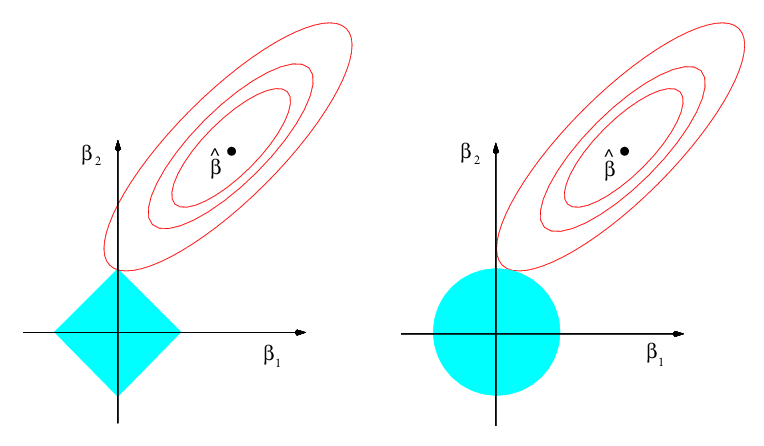
\includegraphics[width=12cm]{lasso}
\end{center}

Červeně jsou vykreslené vrstevnice parabolické jámy neregularizované části ${\sum_{i=1}^{N} (Y_i - \hat{Y}_i)^2}$. Přímo na nějakých osách bude hyperkrychle vrstevnici protínat celkem často, zatímco hypersféra prakticky nikdy (pokud neleží minimum přimo na ose).

U~Lasso může být nežádoucí, že v~případě kolinearity má tendenci volit pouze některé z~příznaků. To se projevuje jako nevýhoda především u~nových dat -- příznak může chybět nebo být sám o~sobě zatížený nějakým šumem. Proto existuje model, elastic net, který má oba regularizační členy ($L_1$ i $L_2$) a kombinuje výhody obou přístupů:
\[
    \RSS_{\lambda_1, \lambda_2}^\Elastic = \sum_{i=1}^{N} (Y_i - \hat{Y}_i)^2
    + \lambda_1 \sum_{i=1}^{p} |w_i|
    + \lambda_2 \sum_{i=1}^{p} w_i^2
\]
\[
    \wh_{\lambda_1, \lambda_2}^\Elastic
    = \argmin_{\we} \RSS_{\lambda_1, \lambda_2}^\Elastic (\we)
\]

\section{Statistické vlastnosti modelů}

V~modelu pro trénovací množinu $\Y = \X\we + \bm{\varepsilon}$ je $\bm{\varepsilon}$ náhodný vektor, z~čehož plyne, že $\Y$ je náhodný vektor, a tedy i $\wh_\lambda$ je náhodný vektor.

\subsection{Očekávaná chyba modelu}

Protože je odhad $\wh_\lambda$ náhodný vektor, můžeme pomocí kvadratické ztrátové funkce zkoumat očekávanou chybu predikce $Y = \we^T\x + \varepsilon$ pomocí $\hat{Y} = \wh_\lambda^T \x$.

\subsubsection{Rozklad očekávané chyby modelu}

Předpokládáme-li, nezávislost trénovací množiny s~testovací množinou, tedy i nezávislost $Y$ a $\hat{Y}$, pak lze očekávanou chybu spočíst jako
\[
    \E L(Y, \hat{Y}) = \E (Y - \hat{Y})^2 = \ldots
    = \textrm{var}\,Y + \E (\hat{Y} - \E Y)^2
    = \sigma^2 + \MSE(\hat{Y})
\]

První člen odpovídá Bayesovské chybě, která je dána náhodností modelu. Druhý člen značíme $\MSE(\hat{Y})$ (mean squared error), který se dá dále dělit na dva členy:
\[
    \MSE(\hat{Y}) = \E (\hat{Y} - \E Y)^2 = \ldots
    = (\E\hat{Y} - \E Y)^2 + \E(\hat{Y} - \E\hat{Y})^2
    = (\text{bias}\,\hat{Y})^2 + \text{var}\,\hat{Y}
\]
kde $\text{bias}\,\hat{Y}$ značí vychýlení odhadu $\hat{Y}$ a $\text{var}\,\hat{Y}$ jeho rozptyl. Finální dekompozice očekávané chyby odhadu je
\[
    \E L(Y, \hat{Y}) = \sigma^2 + (\text{bias}\,\hat{Y})^2 + \text{var}\,\hat{Y}
\]
a skládá se z~neodstranitelné Bayesovské chyby. kvadrátu vychýlení odhadu a rozptylu odhadu.

Tento rozklad je pouze teoretický, v~praxi máme jen celkové MSE, které se snažíme minimalizovat.

\subsection{Bias-variance tradeoff}

Zpravidla s~komplexitou modelu klesá bias (vychýlení), ale roste variance (rozptyl) -- model se přeučuje.

U~hřebenové regrese s~rostoucím regulačním koeficientem klesá rozptyl (regularizace je silnější, odhad $\wh$ je stabilnější), ale zároveň roste vychýlení (koeficienty více ``dusíme'' a jsou systematicky podhodnocované). Takovému chování v~závislosti na hyperparametrech modelu se nazývá bias-variance tradeoff.

V~praxi při ladění hřebenové regresi hledáme optimální $\lambda$, při které je MSE na validační množině $(Y'_i, \x'_i)$ nejmenší. MSE odhadujeme
\[\MSE = \frac{1}{n} \sum_{i=1}^{n} (Y'_i - \wh_\lambda^T\x'_i)^2\]

Při použití hřebenové regrese je rozumné příznaky standardizovat, aby byly rozsahově podobné a penalizované stejně. Příznaky $X_i$ nahradíme
\[
    X_i \leftarrow \frac{X_i - \bar{X}_i}{\sqrt{s_{X_i}^2}},
    \quad \text{kde} \quad
    \bar{X}_i = \tfrac{1}{N} \sum_{i=1}^{N} (X_i)_j
    \quad \text{a} \quad
    s_{X_i}^2 = \tfrac{1}{N-1} \sum_{i=1}^{N} (X_i - \bar{X}_i)^2
\]

\subsection{Nestrannost odhadu v~metodou nejmenších čtverců}

Protože je $\wh_{\text{OLS}}$ bodový odhad (statistika) můžeme zkoumat zda je nestranný. Předpokládáme-li $\E \bm{\varepsilon} = 0$, pak z~linearity střední hodnoty platí
\[
    \E \Y = \E(\X\we + \bm{\varepsilon})
    = \E\X\we + \E\bm{\varepsilon}
    = \X\we
\]
Dále platí
\begin{align*}
    \E\wh_{\text{OLS}}
     & = \E[(\X^T\X)^{-1}\X^T\Y]      \\
     & = (\X^T\X)^{-1}\X^T\E[\Y]      \\
     & = (\X^T\X)^{-1}\X^T\X\we = \we
\end{align*}
Z~čehož plyne
\[
    \E \hat{Y} = \E(\wh_{\text{OLS}}^T\x) = \E(\wh_{\text{OLS}})^T\x = \we^T\x = \E Y
\]
$\hat{Y}$ je tedy nestranným bodovým odhadem $EY$. To znamená, že pro neregularizovanou lineární regresi platí, že je vychýlení nulové:
\[\text{bias}\,\hat{Y} = \E\hat{Y} - \E Y = 0.\]

\section{Logistická regrese}

Logistická regrese predikuje pravděpodobnost jednotlivých hodnot vysvětlované proměnné. Pro binární klasifikaci $Y \in \{0, 1\}$, na kterou se omezíme, tedy vrací pravděpodobnost 1, $P(Y = 1) \in [0, 1]$.

\subsection{Použití pro binární klasifikaci}

\subsubsection{Sigmoida}

V modelu použijeme lineární výraz $\wt\x = w_0 + w_1 x_1 + \ldots + w_p x_p$, který má však obor hodnot na celém $\R$. Tento výraz proto dosadíme do funkce, která je ostře rostoucí a má obor hodnot podmnožinu $[0, 1]$. V logistické regresi volíme sigmoidu
\[f(x) = \frac{e^x}{1+e^x} = \frac{1}{1+e^{-x}}\]
Jedná se o speciální případ logistické funkce
\[f(x) = \frac{L}{1 + e^{-k(x-x_0)}},\]
se supremem $L=1$, koeficientem růstu $k=1$ a středem $x_0 = 0$.

Sigmoida má jako definiční obor celé $\R$ a obor hodnot $(0, 1)$. Na celém definičním oboru je ostře rostoucí, limita pro $x \rightarrow -\infty$ je 0 a pro $x \rightarrow +\infty$ je 1. Také platí, že střed má v bodě 0: $f(0) = \frac{1}{2}$.

\subsubsection{Fungování modelu logistické regrese}

Binární klasifikace vysvětlované proměnné $Y \in \{0,1\}$ s $p$ příznaky $X_1, \ldots, X_p$ logistická regrese provede predikcí pravděpodobnosti
\begin{equation*}
    \text{P} (Y=1 \mid \x, \we ) = \frac{e^{\wtx}}{1 + e^{\wtx}},
\end{equation*}
kde $\x = (1, x_1, \ldots, x_p)$ je vektor hodnot příznaků a $\we = (w_0, \ldots, w_p)$ je vektor koeficientů. Model zvolí 1 když $\text{P} (Y=1 \mid \x, \we ) > 0.5$, jinak predikuje 0.

\subsection{Hranice rozhodnutí}

Hranice rozhodnutí je dána rovnicí
\begin{equation*}
    \text{P} (Y=1 \mid \x, \we ) = 0.5
    \quad \Leftrightarrow \quad
    \wtx = 0
    \quad \Leftrightarrow \quad
    w_0 + w_1 x_1 + \ldots + w_p x_p = 0
\end{equation*}
To odpovídá nadrovině v prostoru $\R^p$. Hranici tedy tvoří lineární varieta dimenze $p-1$.

\subsection{Logistická regrese jako MLE odhad}

Vzhledem k tomu, že u logistické regrese predikujeme pravděpodobnost hodnot proměnné $Y$, nelze vyloženě měřit chybu takových odhadů a následně je minimalizovat jako u lineární regrese. Proto parametry $\we$ odhadujeme MLE (maximum likelihood estimation) metodou maximální věrohodností.

\subsubsection{Myšlenka MLE odhadu}

Pro parametry $\we = (w_0, w_1, \ldots, w_p)$ jsou pravděpodobnosti následující
\begin{align*}
    p_{1}(\x; \we) & = \text{P} (Y=1 \mid \x, \we ) = \frac{e^{\wtx}}{1 + e^{\wtx}} \\
    p_{0}(\x; \we) & = \text{P} (Y=0 \mid \x, \we ) = \frac{1}{1 + e^{\wtx}}
\end{align*}

MLE je takový odhad parametrů, pro které je daná realizace náhodného výběru nejpravděpodobnější (má největší věrohodnost). Metoda maximální věrohodnosti formálně odhaduje hodnotu $\wh$  parametru $\we$, která maximalizuje $L(\we; \X)$ na trénovacích datech $\X = (\x_1, \ldots, \x_N)$, kde $\x_i = (1, x_{i, 1}, \ldots, x_{i, p})$ jsou jednotlivé naměřené hodnoty:
\begin{equation*}
    \wh \in \left\{\argmax_{\we \in \R^{p+1}} L(\we; \X)\right\},
    \quad \text{kde }
    L(\we; \X) = \prod_{i=1}^{N} p_{Y_i}(\x_i; \we)
\end{equation*}

\subsubsection{Sestavení optimalizační úlohy pro trénování}

Pro tuto funkci se snažíme nalézt maximum (nemusí existovat). Před zderivováním se však často vyplatí věrohodnost zlogaritmovat (log-likelihood), který je na $(0, +\infty)$ prostý a ostře rostoucí a tudíž má maximum ve stejném bodě.
\begin{align*}
     & \ell(\we; \X) = \ln L(\we; \X)
    = \sum_{i=1}^{N} \ln p_{Y_i}(\x_i; \we)                                                \\
     & = \sum_{i=1}^{N} Y_i \ln p_{1}(\x_i; \we) + (1 - Y_i) \ln p_{0}(\x_i; \we) = \ldots \\
     & = \sum_{i=1}^{N} \left(Y_i \wt\x_i - \ln(1+e^{\wt\x_i})\right)
\end{align*}

Parciální derivace a gradient vychází
\begin{equation*}
    \pdv{\ell(\we; \X)}{w_j}
    = \sum_{i=1}^{N} \left(Y_i \x_{i,j} - \frac{e^{\wt\x_i} \cdot \x_{i,j}}{1+e^{\wt\x_i}}\right) = \sum_{i=1}^{N} \x_{i,j} \left(Y_i - p_1(\x; \we)\right)
\end{equation*}
\begin{equation*}
    \nabla \ell(\we; \X)
    = \X^T\left(\Y - \bm{P}\right), \quad
    \text{kde } \bm{P} = (p_1(\x_1; \we), \ldots, p_1(\x_N; \we))^T
\end{equation*}

Náš odhad leží v bodě, kde věrohodnost nabývá maxima, což nalezneme položením gradientu nule:
\begin{equation*}
    \nabla \ell(\wh; \X)
    = \X^T\left(\Y - \bm{\hat{P}}\right)
    = \bm{0}
\end{equation*}
Zde neexistuje explicitní řešení a je třeba jej hledat numerickými aproximativními metodami (např. vícerozměrnou Newtonovou metodou lze ukázat, že řešení konverguje k lok. maximu, které je v případě logistické regrese současně globálním maximem).

Výpočet koeficientů logistické regrese je výpočetně náročný. Bez explicitního vzorce je výsledek jen aproximace a je možné, že počítač nic nevrátí (nepodaří se mu nalézt dostatečně dobrá aproximace).

Funkce $\ell(\we; \X)$ také žádné maximum mít nemusí. V takovém případě se numerickou metodou pouze snažíme hledat přibližné řešení $\X^T\left(\Y - \bm{\hat{P}}\right) = \bm{0}$.

\section{Ensemble metody}

Ensemble metody spočívají v~konstrukci velkého množství jednoduchých modelů, jejichž predikce se zkombinují do finálního rozhodnutí.

\subsection{Bagging (bootstrap aggregating)}

Jednou z~metod konstrukce slabých podmodelů (weak learners), je trénování nad náhodným výběrem trénovací množiny. Tím se zajistí rozdílnost podmodelů, jejich pestrost a variabilita. Tato metoda se nazývá bootstrap.

\subsection{Náhodné lesy}

Velmi silným a mocným reprezentantem bagging metody je náhodný les, který agreguje stromy. Tyto stromy jsou zpravidla malé hloubky. Datasety vzniklé bootstrapem způsobí vyšší pestrost stromů, které jsou sami o~sobě velmi citlivé a u~kterých se malá změna dat často projevuje velmi rozdílnými výsledky. Stromům s~rostoucí hloubkou klesá bias, ale roste variance. Kombinací stromů model v~jistém smyslu rozptyl krotí. Díky této stabilitě funguje náhodný les v~praxi velmi dobře.

\subsubsection{Pestrost stromů}

Dalším velmi důležitým krokem v~konstrukci náhodného lesa je náhodný výběr příznaků při každém dělení listu během konstrukce jednotlivých stromů. Algoritmus náhodně volí nějakou podmnožinu příznaků (o~velikosti např. $\sqrt{\cdotp}$, $\log$) mezi kterými hledá ten nelepší split. Silné prediktory budou  stále hodně zastoupené, nicméně v~případě, že se ve výběru nevyskytnou, mají šanci výslednou konstrukci ovlivnit i slabších prediktory (které se mohou nyní vyskytnout i v~kořeni nebo jinde ve vyšších hladinách).

\subsubsection{Predikce}

Náhodný les kombinuje výsledky stromů v~případě klasifikace majoritním hlasováním a v~případě regrese průměrem.

\subsubsection{Shrnutí}

Rozhodovací stromy jsou díky kolektivnímu rozhodování velmi robustní, díky průměrování odolné vůči přeučení (s~rostoucím počtem průměrovaných hodnot klesá rozptyl a roste spolehlivost). Naopak ztrácí interpretovatelnost a trénují se znatelně déle (konstrukce stromů lze však provádět paralelně).

U~náhodného lesa ladíme jako hyperparametry četnost podmodelů, maximální hloubku jednotlivých stromů, počet/poměr náhodně vybraných příznaků při větvení.

\subsection{Boosting}

\subsubsection{Vážené hodnoty u~rozhodovacího stromu}

Princip vážených dat u~rozhodovacího stromu je následovný: Každému prvku $\x_i$ v~trénovací množině přiřadíme nezápornou váhu $w(\x_i)$ tak, že \[\sum_{i=1}^{N} w(\x_i) = 1\]

Při učení se tak význam vah u~výpočtu informačního zisku trochu mění.
\[
    IG(\D) = H(\D) - t_0 H(\D_0) - t_1 H(\D_1),
\]

kde $\D_0, \D_1$ jsou příslušné podmnožiny $\D$, jsou nyní koeficienty definované jako
\begin{equation*}
    t_0 = \frac{\sum_{\x \in \D_0} w(\x)}{\sum_{\x \in \D} w(\x)}
    \quad \text{a} \quad
    t_1 = \frac{\sum_{\x \in \D_1} w(\x)}{\sum_{\x \in \D} w(\x)}.
\end{equation*}

Takhle naučený strom klade větší důraz na to, aby správně predikoval datové body s~vyšší váhou.

\subsubsection{AdaBoost}

AdaBoost podobně jako bagging konstruuje velké množství stromů, jejichž výsledky pro finální predikci kombinuje. Na rozdíl od náhodného lesa však spolu vybudované stromy souvisí. Stromy se konstruují sekvenčně, přičemž každý strom v~posloupnosti se soustředí na ty datové body, ve kterých předchozí strom chyboval (zvýší jim váhu).

\paragraph{Konstrukce stromů}

V~algoritmu se vyskytuje hodnota $\lambda$ (learning rate), která v~případě, že je menší než jedna trénování zpomaluje a zabraňuje přeučení. Pro $\lambda \ge 1$ je konstrukce významných stromů rychlejší, ale zároveň volatilní (zběsile řeší ``aktuální'' problém, kterým rychleji vznikají špatně klasifikované hodnoty, na které se nesoustředil).

\begin{algorithm}[H]
    \renewcommand{\thealgorithm}{}
    \caption{AdaBoost}
    \begin{algorithmic}[1]
        \Require
        \Statex Trénovací data $\D$.
        \Statex Learning rate $\lambda \ge 0$.
        \Statex
        \State Přiřaď všem datovým bodům váhu $w_i = \frac{1}{N}$.
        \State Polož $m = 1$ (indexuje stromy v~posloupnosti).
        \While{$m \le \texttt{n\_estimators}$}
        \State Natrénuj strom $T^{(m)}$ s~váhami $w_i$.
        \State Spočítej součet vah $e^{(m)}$ špatně klasifikovaných hodnot v~$T^{(m)}$.
        \State Pokud je $e^{(m)} = 0$, skonči.
        \State Polož \[\alpha^{(m)} = \lambda \log\frac{1 - e^{(m)}}{e^{(m)}}.\]
        \State Špatně klasifikovaným prvkům v~$T^{(m)}$ přiřaď nové váhy
        \[w_i \leftarrow w_i \exp(\alpha^{(m)}).\]
        \State Váhy znormalizuj, aby součet byl 1, a inkrementuj $m$.
        \EndWhile
        \State \Return $T^{(1)}, T^{(2)}, \ldots, T^{(m)}$
    \end{algorithmic}
\end{algorithm}

\paragraph{O~regularizaci}

Regularizaci většinou doprovází nějaký tradeoff. V~případě AdaBoostu se jedná o~pomalejší trénování (je potřeba víc stromů), nebo v~případě hřebenové regrese způsobuje vychýlení odhadu $\wh$.

\paragraph{Predikce}

Model každému stromu $T^{(m)}$ přiřadí váhu $\alpha^{(m)}$ a při klasifikaci spočte $W_1$ součet vah stromů, které predikují 1, a $W_0$ součet vah stromů, které predikují 0. Ve finále predikuje tu hodnotu, která má mezi všemi stromy vyšší celkovou váhu.

Existuje i verze AdaBoostu pro multiclass klasifikaci: AdaBoost-SAMME, a pro regresi: AdaBoost.R2. AdaBoost nemusí nutně používat stromy. Umí používat jakýkoliv model, který umí správně pracovat s~váženými datovými body.

\documentclass[../main.tex]{subfiles}
\begin{document}
\section{Evaluace modelů}

Jedna z klíčových aspektů strojového učení je, aby natrénovaný model byl schopný generalizace -- fungovat dobře na nových vstupech.

Při trénování můžeme natrénovat celou řadu modelů (např. ze stejné rodiny ale s různými sadami hyperparametrů). Pro to, abychom mohli modely porovnat, potřebujeme mít nějakou kvantitativní míru výkonnosti -- metriku. To jakou zvolíme často záleží na charakteru problému. Někdy chceme minimalizovat drobné chyby, někdy celkovou chybovost, apod.

\subsection{Ztrátová funkce}

Uvažujme model natrénovaný na vstupu $\X$ s vysvětlovanou proměnnou $Y$. Takový model zpravidla není dokonalý a pro $\X$ predikuje nějaké $\hat{Y} \equiv \hat{Y}(\X)$. Funkci $L$, měřící chybu této predikce, nazýváme ztrátovou funkcí (loss function).

\paragraph{Regrese} V případě regrese je typická kvadratická ztrátová funkce (squared error): \[L(Y, \hat{Y}) = (Y - \hat{Y})^2, \] případně $L_1$  ztrátová funkce měřící absolutní chybu (absolute error): \[L(Y, \hat{Y}) = |Y - \hat{Y}|.\]

\paragraph{Klasifikace} U binární klasifikace se často odhaduje pravděpodobnost \[\hat{p} = \hat{P}(Y=1 \mid \X = \x),\] pro kterou se nabízí následující ztrátová funkce (binary cross-entropy loss function) \[L(Y, \hat{Y}) = -Y\log\hat{p} - (1-Y)\log(1-\hat{p})\]

\subsubsection{Trénovací chyba}

Při trénování se snažíme minimalizovat průměrnou hodnotu ztrátové chyby přes všechny prvky v trénovací množině (trénovací chybu, test error): \[\overline{\err}_\train = \mathcal{L} = \frac{1}{N} \sum_{i=1}^{N} L(Y_i, \hat{Y}(\x_i))\]

V případě regrese se tedy bude jednat například o
\[
    \MSE_\train = \frac{1}{N} \sum_{i=1}^{N} (Y - \hat{Y})^2
    \quad \text{nebo} \quad
    \MAE_\train = \frac{1}{N} \sum_{i=1}^{N} |Y - \hat{Y}|
\]

A u binární klasifikaci o
\[
    \mathcal{L} = \frac{1}{N} \sum_{i=1}^{N}
    \left[
        - Y_i\log\hat{p}(\x_i) - (1-Y_i)\log(1-\hat{p}(\x_i))]
    \right]
\]

Řešení minimalizující trénovací chybu (test error) lze u některých modelů spočíst explicitně (closed-form solution), např. u lin. regrese. Pro většinu modelů to nelze a musíme jej počítat numericky iterativními metodami (např. gradientním sestupem).

\subsubsection{Testovací chyba}

Testovací chyba (test error) je střední chyba na novém vstupu $\X$ při dané trénovací množině $\D$:
\[
    \Err_\D = \E (L(Y, \hat{Y}(\X)) \mid \D)
\]
kterou můžeme odhadnout
\[
    \overline{\err}_\test = \frac{1}{N_\test} \sum_{i=1}^{N_\test} (L(Y_i, \hat{Y}(\x_i))
\]

Nejobecnější mírou schopnosti modelu generalizovat je očekávaná testovací chyba (expected test error), která je střední hodnotou testovací chyby pro náhodný výběr trénovací množiny $\D$:
\[
    \Err = \E (\Err_\D) = \E (L(Y, \hat{Y}(\X)))
\]
Jedná se tedy odhad $\Err_\D$ s neznámým $\D$.

\subsection{Evaluační scénáře}

Z pohledu evaluace máme dva úkoly:
\begin{itemize}
    \item Výběr modelu - odhadnout chybu různých modelů za účelem výběru nejlepšího.
    \item Ohodnocení modelu - odhadnout testovací chybu finálního modelu.
\end{itemize}

\subsubsection{Hold-out}

Pokud máme dostatek dat, dělíme data na část
\begin{itemize}
    \item Trénovací - k natrénování konkrétních modelů.
    \item Validační - k výběru nejlepší sady hyperparametrů.
    \item Testovací - k odhadu testovací chyby, kterou očekáváme na nových datech.
\end{itemize}
Pro získání neoptimistického odhadu výkonnosti modelu, musí být testovací část skutečně nový vstup, který nijak neovlivnil parametry ani volbu modelu.

\subsubsection{k-fold cross-validation}

Pokud nemáme dostatek dat, je často nerozumné je dělit na trénovací, validační a testovací. Vedlo by to na nedostatek dat pro správně natrénovaní, dobrou volbu správného modelu a spolehlivého odhadu testovací chyby.

S křížovou validací se obejdeme bez validační množiny.
\begin{algorithm}[H]
    \renewcommand{\thealgorithm}{}
    \caption{Cross-validation}
    \begin{algorithmic}[1]
        \Require $2 \le k \le N$
        \item Trénovací data $\D$ rozděl na $k$ podobně velkých podmnožin $\D_1, \ldots, \D_k$.
        \item Pro $j = 1, \ldots, k$ natrénuj model s danými hyperparametry na $\D \setminus \D_j$.
        \item Na $\D_j$ odhadni chybu modelu $e_j$.
        \item \Return cross-validation error
        \[\hat{e} = \frac{1}{k} \sum_{i=1}^{k} e_i\]
    \end{algorithmic}
\end{algorithm}

Takto odhadneme cross-validační chybu pro všechny uvažované sady hyperparametrů a zvolíme model s nejnižší takovou chybou. Zvolený model s nejlepšími hyperparametry natrénujeme na celé množině $\D$.

Volba $k$ je kvůli výpočetním nárokům obvykle malá (5, 10). Pro velmi malé datasety může však být únosná i volba $k=N$ (leave-one-out cross-validation).

\paragraph{Cross-validation error} Cross-validation error je odhad očekávané testovací chyby $\Err$ a ne testovací chyby $\Err_\D$.

Při skutečně malém datasetu je možné zvolit dvoustupňovou křížovou validaci, která si neodkládá testovací sadu, ale zanořuje se s křížovou validací o jednu stupeň níž, přičemž vnitřní cross-validační chyba se používá pro výběr modelu a vnější pro odhad očekávané chyby.

Vnější cross-validation chyba je pouze jedna (``společná'') a odpovídá očekávané testovací chybě celé procedury pro výběr nejlepšího
modelu, ale nejlepší model teprve musíme získat (natrénování zvoleného modelu na celé množině $\D$).

\paragraph{Finální model} Ve všech metodách lze po výsledném odhadu testovací chyby přetrénovat nejlepší model na celém datasetu a pro odhad výkonnosti použít testovací chybu, resp. očekávanou testovací chybu, z předchozího kroku. U hold-out lze před evaluací na trénovacích datech ještě přetrénovat model na (trénovací + validační) množině.

\subsection{Evaluace regrese}

Nejčastější volba ztrátové funkce u regresních úloh je MSE (mean squared error) nebo MAE (mean absolute error):
\[
    \MSE = \frac{1}{N} \sum_{i=1}^{N} (Y_i - \hat{Y}_i)^2
    \qquad
    \MAE = \frac{1}{N} \sum_{i=1}^{N} |Y_i - \hat{Y}_i|
\]
Zatímco MSE je citlivější na velká residua, MAE se spíše soustředí na celkovou chybu a odlehlým hodnotám se chová ``spravedlivě''. Jednotky MSE jsou v kvadrátech, proto se také často udává přeškálované RMSE, které má interpretovatelné jednotky vysvětlované proměnné:
\[
    \RMSE = \sqrt{\frac{1}{N} \sum_{i=1}^{N} (Y_i - \hat{Y}_i)^2}
\]

Pro nezáporné hodnoty lze použít ztrátovou funkcí RMSLE, které se soustředí na relativní míru odchylek:
\[
    \RMSLE = \sqrt{\frac{1}{N} \sum_{i=1}^{N} (\log Y_i - \log \hat{Y}_i)^2}
    = \sqrt{\frac{1}{N} \sum_{i=1}^{N} \log^2 \frac{Y_i}{\hat{Y}_i}}
\]

Koeficient determinace $R^2$ (coefficient of determination) vyjadřuje podíl variability cílové proměnné, kterou model vysvětluje:
\[
    R^2 = 1 - \frac{\RSS}{\TSS}
    = \frac{
        \sum_{i=1}^{N} (\log Y_i - \log \hat{Y}_i)^2
    }{
        \sum_{i=1}^{N} (\log Y_i - \log \bar{Y})^2
    },
\]
kde TSS je total sum of squares (RSS modelu, který predikuje $\bar{Y}$ pro každý datový bod).

\subsection{Evaluace klasifikace}

\paragraph{Matice záměn}

U klasifikace je konstrukce a interpretace ztrátových funkcí obecně problematické. Využívá se proto matice záměn:
{\def\arraystretch{1.5}
\begin{center}
    \begin{tabular}{ c c | c c | c }
                 &               & \multicolumn{2}{c|}{Skutečnost}                       \\
                 &               & $Y = 1$                         & $Y=0$ & $\Sigma$    \\
        \hline
        Predikce & $\hat{Y} = 1$ & TP                              & FP    & $\hat{N}_+$ \\
                 & $\hat{Y} = 0$ & FN                              & TN    & $\hat{N}_-$ \\
        \hline
                 & $\Sigma$      & $N_+$                           & $N_-$ & $N$
    \end{tabular}
\end{center}}
(T/F - True/False; P/N - Positive/Negative)

Z matice záměn můžeme vyvodit následující míry:
{\def\arraystretch{2}
\begin{center}
    \begin{tabular}{ c c | c c }
                                   &               & \multicolumn{2}{c}{Skutečnost}                                 \\
        $\text{P}(\hat{Y} \mid Y)$ &               & $Y = 1$                        & $Y=0$                         \\
        \hline
        Predikce                   & $\hat{Y} = 1$ & TPR = $\frac{\text{TP}}{N_+}$  & FPR = $\frac{\text{FP}}{N_+}$ \\
                                   & $\hat{Y} = 0$ & FNR = $\frac{\text{FN}}{N_-}$  & TNR = $\frac{\text{TN}}{N_-}$ \\
    \end{tabular}
\end{center}}
\begin{itemize}
    \item True positive rate (TPR): senzitivita (recall).
    \item False positive rate (FPR): type I error rate.
    \item False negative rate (FNR): type II error rate.
    \item True negative rate (TNR): specificita (specificity).
\end{itemize}
Často používanou mírou (např. ve výpočtu $F_1$) je také odhad $P(Y = 1 \mid \hat{Y} = 1)$ (precision):
\[\text{PPV} = \frac{\text{TP}}{\hat{N}_+}\]

\subsubsection{Evaluační míry binární klasifikace}

Nejpoužívanější mírou je přesnost (accuracy) -- odhad $P(Y = \hat{Y})$:
\[\text{ACC} = \frac{\text{TP} + \text{TN}}{N}\]
Tato míra však není spolehlivá pro nevybalancovaná data, kdy modelu stačí predikovat pouze majoritní třídu. V takovém případě se používá $F_1$ score:
\[F_1 = \frac{2}{\text{PPV}^{-1} + \text{TPR}^{-1}},\]
kde hodnota $P(Y=1)$ je velmi malá.

\subsubsection{ROC a AUC}

Modely binární klasifikace často odhadují $p(\X) = P(Y = 1 \mid \X)$ a predikují
\[\hat{Y} = \mathds{1}_{\hat{p} > 0.5}\]

Hodnotu 0.5 však můžeme parametrizovat pomoc $\tau \in [0, 1]$ a získat tak pro různé hranice různé predikce:
\[\hat{Y}_\tau = \mathds{1}_{\hat{p} > \tau}\]

\paragraph{ROC}

S hodnotou $\tau$ od 0 do 1 se různě mění TPR a FPR, jejichž vztah lze vykreslit a následně dále zkoumat pomocí ROC křivky (receiver operating characteristic curve).
\begin{center}
    \small
    \begin{tikzpicture}[scale=1.1]
        \begin{axis}[
                xlabel={FPR},
                ylabel={TPR},
                title={ROC křivka},
                xmin=0, xmax=1,
                ymin=0, ymax=1,
                legend pos=south east,
            ]

            \addplot[smooth, color=blue] coordinates {(0,0) (0.1,0.6) (0.2,0.75) (0.3,0.8) (0.6,0.9) (0.8,0.95) (1,1)};
            \addlegendentry{ROC křivka}

            \addplot[smooth, color=red, dashed] coordinates {(0,0) (1,1)};
            \addlegendentry{náhodné predikce}

        \end{axis}
    \end{tikzpicture}
\end{center}
Pro dobrý model se křivka přimyká k levé a horní ose (strmě roste).

\paragraph{AUC}

Kvalita modelu, pro kterou máme ROC křivku, vyhodnocujeme plochou pod křivkou AUC (area under the curve). Model s náhodnými predikcemi má AUC = 0.5, dokonalý model by měl AUC = 1.

\begin{center}
    \small
    \begin{tikzpicture}[scale=1.1]
        \begin{axis}[
                xlabel={FPR},
                ylabel={TPR},
                title={ROC křivka s AUC},
                xmin=0, xmax=1,
                ymin=0, ymax=1,
                legend pos=south east,
            ]

            \addplot[fill=blue, fill opacity=0.15, smooth, area legend, draw=none]  coordinates {(0,0) (0.1,0.6) (0.2,0.75) (0.3,0.8) (0.6,0.9) (0.8,0.95) (1,1)} \closedcycle;

            \addplot[smooth, color=blue, line legend] coordinates {(0,0) (0.1,0.6) (0.2,0.75) (0.3,0.8) (0.6,0.9) (0.8,0.95) (1,1)};

            \addplot[smooth, color=red, dashed, line legend] coordinates {(0,0) (1,1)};
            \legend{AUC = 0.85, ROC křivka, náhodné predikce}

        \end{axis}
    \end{tikzpicture}
\end{center}

\end{document}

\section{Nesupervizované učení}

Nesupervizované učení se zabývá problematikou neoznačených dat. Cílem je tedy datům porozumět, případně odhalit nějakou vnitřní strukturu. To většinou znamená odhalit nějaké omezené oblasti v prostoru příznaků, ve kterých se data vyskytují častěji (data se zpravidla nevyskytují náhodně, často tvoří nějaké shluky). Bývají nějakým způsobem lokalizovaná (např. v nějakých méně dim. oblastech, apod.).

Obecným problémem je, že zpočátku typicky o datech nemáme žádnou informaci. Tu se snažíme různými metodami z dat extrahovat. Na rozdíl od nesupervizového učení zde není jasný postup, nebo přímočarý způsob, jak úspěšnost řešení vyhodnocovat.

\paragraph{Z pohledu teorie pravděpodobnosti} Uvažujme realizaci náhodného vektoru $\X = (X_1, \ldots, X_p)^T$ v prostoru $\calX$, které je v případě binárních příznaků $\calX = \{0,1\}^p$ a v případě spojitých příznaků $\calX = \R^p$.

Porozuměním vnitřní struktuře znamená porozumění rozdělení $\X$ tak, že jsme schopni spolehlivě predikovat pravděpodobnost $\text{P}(\X \in O)$, kde $O$ je nějakou zajímavou podmnožinou $\calX$.

Odhadujeme tedy pravděpodobnostní hustotu $f_{\X}(x_1, \ldots, x_p)$, respektive pravděpodobnostní funkci $\text{P}_{\X}(X_1 = x_1, \ldots, X_p = x_p)$.

\section{Shluková analýza}

Shluková analýza (clustering) je metoda nesupervizovaného učení, která rozřadí data do nějakých shluků tak, aby byly blízké body v~jednom shluku a vzdálené v~různých. Jak přesně formalizovat takovou úlohu je problematické, proto může mít různá řešení v~závislosti na tom, jak definujeme vzdálenost.

\paragraph{Vzdálenost} Pro připomenutí, definice metriky byla zevedena v~sekci \ref{sec:metrika}.

\paragraph{Formalizace úlohy shlukování} Úloha na vstupu dostane metrický prostor $\calX$ se vzdáleností $d$, množinu dat $\D \subset \calX$ a počet požadovaných shluků $k$. Na výstupu se požaduje nějaký rozklad množiny $\D$ na $k$ shluků. To znamená $C_1, \ldots, C_k \subset \D$, kde $C_i \neq C_j$ pro všechna $i \neq j$, přičemž \[\D = \bigcup_{i=1}^{k} C_i.\]

\subsection{Hierarchické shlukování}

Hierarchické shlukování používá hladový aglomerativní přístup popsaný v~následujícím algoritmu.

\begin{algorithm}[H]
    \renewcommand{\thealgorithm}{}
    \caption{Hierarchické shlukování}
    \begin{algorithmic}[1]
        \Require
        \Statex Množina dat $\D$ a metrika pro vzdálenost shluků.
        \Statex Požadovaný počet shluků $k$ (jinak $k=1$).
        \Statex
        \State Uvažuj každý bod jako jednoprvkový shluk (celkem $|\D|$ shluků).
        \While{počet shluků $> k$}
        \State Nalezni dva nejbližší shluky.
        \State Tyto dva shluky spoj do jednoho.
        \EndWhile
    \end{algorithmic}
\end{algorithm}

\subsubsection{Měření vzdáleností shluků}

Po volbě metriky dvou bodů $d(a, b)$ je ještě nutné zvollit vzdálenost dvou shluků $D(A, B)$. Obvykle se použije jedna z~následujících:
\begin{itemize}

    \item Single linkage, který generuje dlouhé řetězce
          \[
              D(A, B) = \min_{\x \in A,\y \in B} d(\x, \y).
          \]

    \item Complete linkage, který generuje kompaktní buňky
          \[
              D(A, B) = \max_{\x \in A,\y \in B} d(\x, \y).
          \]

    \item Average linkage, který měří podle průměrné vzdálenosti všech bodů
          \[
              D(A, B) = \frac{1}{|A| |B|} \sum_{\x \in A,\y \in B} d(\x, \y).
          \]

    \item Wardova metoda (pouze pro $\calX = \R^p$), která minimalizuje nárůst vnitřního rozptylu buněk
          \[
              D(A, B) = \sum_{\x \in A \cup B} \|\x - \bm{\bar{x}}_{A \cup B} \|^2
              - \sum_{\x \in A} \|\x - \bm{\bar{x}}_A \|^2
              - \sum_{\x \in B} \|\x - \bm{\bar{x}}_B \|^2,
          \]
          kde $\bm{\bar{x}}_S$ značí geometrický střed (centroid) shluku $S$.

\end{itemize}

\subsubsection{Dendrogram}

Celý proces aglomerativního shlukování lze reprezentovat dendrogramem. To je strom, který má v~listech počáteční jednoprvkové shluky a ve vrcholech spojení. Obvykle algoritmus běží, dokud nespojí všechny shluky, v~takovém případě má v~kořeni finální shluk. Strom se vykresluje tak, že listy jsou ve výšce 0 a jednotlivé vrcholy ve výšce podle vzdálenosti shluků, které se v~daném bodě spojily (vzdálenost, kterou musely ``překonat'').

\begin{center}
    \scalebox{0.7}{%% Creator: Matplotlib, PGF backend
%%
%% To include the figure in your LaTeX document, write
%%   \input{<filename>.pgf}
%%
%% Make sure the required packages are loaded in your preamble
%%   \usepackage{pgf}
%%
%% Also ensure that all the required font packages are loaded; for instance,
%% the lmodern package is sometimes necessary when using math font.
%%   \usepackage{lmodern}
%%
%% Figures using additional raster images can only be included by \input if
%% they are in the same directory as the main LaTeX file. For loading figures
%% from other directories you can use the `import` package
%%   \usepackage{import}
%%
%% and then include the figures with
%%   \import{<path to file>}{<filename>.pgf}
%%
%% Matplotlib used the following preamble
%%   \def\mathdefault#1{#1}
%%   \everymath=\expandafter{\the\everymath\displaystyle}
%%   
%%   \usepackage{fontspec}
%%   \setmainfont{DejaVuSerif.ttf}[Path=\detokenize{/home/chutommy/miniconda3/envs/viz/lib/python3.10/site-packages/matplotlib/mpl-data/fonts/ttf/}]
%%   \setsansfont{DejaVuSans.ttf}[Path=\detokenize{/home/chutommy/miniconda3/envs/viz/lib/python3.10/site-packages/matplotlib/mpl-data/fonts/ttf/}]
%%   \setmonofont{DejaVuSansMono.ttf}[Path=\detokenize{/home/chutommy/miniconda3/envs/viz/lib/python3.10/site-packages/matplotlib/mpl-data/fonts/ttf/}]
%%   \makeatletter\@ifpackageloaded{underscore}{}{\usepackage[strings]{underscore}}\makeatother
%%
\begingroup%
\makeatletter%
\begin{pgfpicture}%
\pgfpathrectangle{\pgfpointorigin}{\pgfqpoint{8.000000in}{5.000000in}}%
\pgfusepath{use as bounding box, clip}%
\begin{pgfscope}%
\pgfsetbuttcap%
\pgfsetmiterjoin%
\definecolor{currentfill}{rgb}{1.000000,1.000000,1.000000}%
\pgfsetfillcolor{currentfill}%
\pgfsetlinewidth{0.000000pt}%
\definecolor{currentstroke}{rgb}{1.000000,1.000000,1.000000}%
\pgfsetstrokecolor{currentstroke}%
\pgfsetdash{}{0pt}%
\pgfpathmoveto{\pgfqpoint{0.000000in}{0.000000in}}%
\pgfpathlineto{\pgfqpoint{8.000000in}{0.000000in}}%
\pgfpathlineto{\pgfqpoint{8.000000in}{5.000000in}}%
\pgfpathlineto{\pgfqpoint{0.000000in}{5.000000in}}%
\pgfpathlineto{\pgfqpoint{0.000000in}{0.000000in}}%
\pgfpathclose%
\pgfusepath{fill}%
\end{pgfscope}%
\begin{pgfscope}%
\pgfsetbuttcap%
\pgfsetmiterjoin%
\definecolor{currentfill}{rgb}{1.000000,1.000000,1.000000}%
\pgfsetfillcolor{currentfill}%
\pgfsetlinewidth{0.000000pt}%
\definecolor{currentstroke}{rgb}{0.000000,0.000000,0.000000}%
\pgfsetstrokecolor{currentstroke}%
\pgfsetstrokeopacity{0.000000}%
\pgfsetdash{}{0pt}%
\pgfpathmoveto{\pgfqpoint{1.000000in}{0.550000in}}%
\pgfpathlineto{\pgfqpoint{7.200000in}{0.550000in}}%
\pgfpathlineto{\pgfqpoint{7.200000in}{4.400000in}}%
\pgfpathlineto{\pgfqpoint{1.000000in}{4.400000in}}%
\pgfpathlineto{\pgfqpoint{1.000000in}{0.550000in}}%
\pgfpathclose%
\pgfusepath{fill}%
\end{pgfscope}%
\begin{pgfscope}%
\definecolor{textcolor}{rgb}{0.000000,0.000000,0.000000}%
\pgfsetstrokecolor{textcolor}%
\pgfsetfillcolor{textcolor}%
\pgftext[x=1.193750in,y=0.452778in,,top]{\color{textcolor}{\sffamily\fontsize{12.000000}{14.400000}\selectfont\catcode`\^=\active\def^{\ifmmode\sp\else\^{}\fi}\catcode`\%=\active\def%{\%}(7)}}%
\end{pgfscope}%
\begin{pgfscope}%
\definecolor{textcolor}{rgb}{0.000000,0.000000,0.000000}%
\pgfsetstrokecolor{textcolor}%
\pgfsetfillcolor{textcolor}%
\pgftext[x=1.581250in,y=0.452778in,,top]{\color{textcolor}{\sffamily\fontsize{12.000000}{14.400000}\selectfont\catcode`\^=\active\def^{\ifmmode\sp\else\^{}\fi}\catcode`\%=\active\def%{\%}(8)}}%
\end{pgfscope}%
\begin{pgfscope}%
\definecolor{textcolor}{rgb}{0.000000,0.000000,0.000000}%
\pgfsetstrokecolor{textcolor}%
\pgfsetfillcolor{textcolor}%
\pgftext[x=1.968750in,y=0.452778in,,top]{\color{textcolor}{\sffamily\fontsize{12.000000}{14.400000}\selectfont\catcode`\^=\active\def^{\ifmmode\sp\else\^{}\fi}\catcode`\%=\active\def%{\%}41}}%
\end{pgfscope}%
\begin{pgfscope}%
\definecolor{textcolor}{rgb}{0.000000,0.000000,0.000000}%
\pgfsetstrokecolor{textcolor}%
\pgfsetfillcolor{textcolor}%
\pgftext[x=2.356250in,y=0.452778in,,top]{\color{textcolor}{\sffamily\fontsize{12.000000}{14.400000}\selectfont\catcode`\^=\active\def^{\ifmmode\sp\else\^{}\fi}\catcode`\%=\active\def%{\%}(5)}}%
\end{pgfscope}%
\begin{pgfscope}%
\definecolor{textcolor}{rgb}{0.000000,0.000000,0.000000}%
\pgfsetstrokecolor{textcolor}%
\pgfsetfillcolor{textcolor}%
\pgftext[x=2.743750in,y=0.452778in,,top]{\color{textcolor}{\sffamily\fontsize{12.000000}{14.400000}\selectfont\catcode`\^=\active\def^{\ifmmode\sp\else\^{}\fi}\catcode`\%=\active\def%{\%}(10)}}%
\end{pgfscope}%
\begin{pgfscope}%
\definecolor{textcolor}{rgb}{0.000000,0.000000,0.000000}%
\pgfsetstrokecolor{textcolor}%
\pgfsetfillcolor{textcolor}%
\pgftext[x=3.131250in,y=0.452778in,,top]{\color{textcolor}{\sffamily\fontsize{12.000000}{14.400000}\selectfont\catcode`\^=\active\def^{\ifmmode\sp\else\^{}\fi}\catcode`\%=\active\def%{\%}(7)}}%
\end{pgfscope}%
\begin{pgfscope}%
\definecolor{textcolor}{rgb}{0.000000,0.000000,0.000000}%
\pgfsetstrokecolor{textcolor}%
\pgfsetfillcolor{textcolor}%
\pgftext[x=3.518750in,y=0.452778in,,top]{\color{textcolor}{\sffamily\fontsize{12.000000}{14.400000}\selectfont\catcode`\^=\active\def^{\ifmmode\sp\else\^{}\fi}\catcode`\%=\active\def%{\%}(4)}}%
\end{pgfscope}%
\begin{pgfscope}%
\definecolor{textcolor}{rgb}{0.000000,0.000000,0.000000}%
\pgfsetstrokecolor{textcolor}%
\pgfsetfillcolor{textcolor}%
\pgftext[x=3.906250in,y=0.452778in,,top]{\color{textcolor}{\sffamily\fontsize{12.000000}{14.400000}\selectfont\catcode`\^=\active\def^{\ifmmode\sp\else\^{}\fi}\catcode`\%=\active\def%{\%}(8)}}%
\end{pgfscope}%
\begin{pgfscope}%
\definecolor{textcolor}{rgb}{0.000000,0.000000,0.000000}%
\pgfsetstrokecolor{textcolor}%
\pgfsetfillcolor{textcolor}%
\pgftext[x=4.293750in,y=0.452778in,,top]{\color{textcolor}{\sffamily\fontsize{12.000000}{14.400000}\selectfont\catcode`\^=\active\def^{\ifmmode\sp\else\^{}\fi}\catcode`\%=\active\def%{\%}(9)}}%
\end{pgfscope}%
\begin{pgfscope}%
\definecolor{textcolor}{rgb}{0.000000,0.000000,0.000000}%
\pgfsetstrokecolor{textcolor}%
\pgfsetfillcolor{textcolor}%
\pgftext[x=4.681250in,y=0.452778in,,top]{\color{textcolor}{\sffamily\fontsize{12.000000}{14.400000}\selectfont\catcode`\^=\active\def^{\ifmmode\sp\else\^{}\fi}\catcode`\%=\active\def%{\%}(15)}}%
\end{pgfscope}%
\begin{pgfscope}%
\definecolor{textcolor}{rgb}{0.000000,0.000000,0.000000}%
\pgfsetstrokecolor{textcolor}%
\pgfsetfillcolor{textcolor}%
\pgftext[x=5.068750in,y=0.452778in,,top]{\color{textcolor}{\sffamily\fontsize{12.000000}{14.400000}\selectfont\catcode`\^=\active\def^{\ifmmode\sp\else\^{}\fi}\catcode`\%=\active\def%{\%}(5)}}%
\end{pgfscope}%
\begin{pgfscope}%
\definecolor{textcolor}{rgb}{0.000000,0.000000,0.000000}%
\pgfsetstrokecolor{textcolor}%
\pgfsetfillcolor{textcolor}%
\pgftext[x=5.456250in,y=0.452778in,,top]{\color{textcolor}{\sffamily\fontsize{12.000000}{14.400000}\selectfont\catcode`\^=\active\def^{\ifmmode\sp\else\^{}\fi}\catcode`\%=\active\def%{\%}(7)}}%
\end{pgfscope}%
\begin{pgfscope}%
\definecolor{textcolor}{rgb}{0.000000,0.000000,0.000000}%
\pgfsetstrokecolor{textcolor}%
\pgfsetfillcolor{textcolor}%
\pgftext[x=5.843750in,y=0.452778in,,top]{\color{textcolor}{\sffamily\fontsize{12.000000}{14.400000}\selectfont\catcode`\^=\active\def^{\ifmmode\sp\else\^{}\fi}\catcode`\%=\active\def%{\%}(4)}}%
\end{pgfscope}%
\begin{pgfscope}%
\definecolor{textcolor}{rgb}{0.000000,0.000000,0.000000}%
\pgfsetstrokecolor{textcolor}%
\pgfsetfillcolor{textcolor}%
\pgftext[x=6.231250in,y=0.452778in,,top]{\color{textcolor}{\sffamily\fontsize{12.000000}{14.400000}\selectfont\catcode`\^=\active\def^{\ifmmode\sp\else\^{}\fi}\catcode`\%=\active\def%{\%}(22)}}%
\end{pgfscope}%
\begin{pgfscope}%
\definecolor{textcolor}{rgb}{0.000000,0.000000,0.000000}%
\pgfsetstrokecolor{textcolor}%
\pgfsetfillcolor{textcolor}%
\pgftext[x=6.618750in,y=0.452778in,,top]{\color{textcolor}{\sffamily\fontsize{12.000000}{14.400000}\selectfont\catcode`\^=\active\def^{\ifmmode\sp\else\^{}\fi}\catcode`\%=\active\def%{\%}(15)}}%
\end{pgfscope}%
\begin{pgfscope}%
\definecolor{textcolor}{rgb}{0.000000,0.000000,0.000000}%
\pgfsetstrokecolor{textcolor}%
\pgfsetfillcolor{textcolor}%
\pgftext[x=7.006250in,y=0.452778in,,top]{\color{textcolor}{\sffamily\fontsize{12.000000}{14.400000}\selectfont\catcode`\^=\active\def^{\ifmmode\sp\else\^{}\fi}\catcode`\%=\active\def%{\%}(23)}}%
\end{pgfscope}%
\begin{pgfscope}%
\pgfsetbuttcap%
\pgfsetroundjoin%
\definecolor{currentfill}{rgb}{0.000000,0.000000,0.000000}%
\pgfsetfillcolor{currentfill}%
\pgfsetlinewidth{0.803000pt}%
\definecolor{currentstroke}{rgb}{0.000000,0.000000,0.000000}%
\pgfsetstrokecolor{currentstroke}%
\pgfsetdash{}{0pt}%
\pgfsys@defobject{currentmarker}{\pgfqpoint{-0.048611in}{0.000000in}}{\pgfqpoint{-0.000000in}{0.000000in}}{%
\pgfpathmoveto{\pgfqpoint{-0.000000in}{0.000000in}}%
\pgfpathlineto{\pgfqpoint{-0.048611in}{0.000000in}}%
\pgfusepath{stroke,fill}%
}%
\begin{pgfscope}%
\pgfsys@transformshift{1.000000in}{0.550000in}%
\pgfsys@useobject{currentmarker}{}%
\end{pgfscope}%
\end{pgfscope}%
\begin{pgfscope}%
\definecolor{textcolor}{rgb}{0.000000,0.000000,0.000000}%
\pgfsetstrokecolor{textcolor}%
\pgfsetfillcolor{textcolor}%
\pgftext[x=0.814412in, y=0.497238in, left, base]{\color{textcolor}{\sffamily\fontsize{10.000000}{12.000000}\selectfont\catcode`\^=\active\def^{\ifmmode\sp\else\^{}\fi}\catcode`\%=\active\def%{\%}0}}%
\end{pgfscope}%
\begin{pgfscope}%
\pgfsetbuttcap%
\pgfsetroundjoin%
\definecolor{currentfill}{rgb}{0.000000,0.000000,0.000000}%
\pgfsetfillcolor{currentfill}%
\pgfsetlinewidth{0.803000pt}%
\definecolor{currentstroke}{rgb}{0.000000,0.000000,0.000000}%
\pgfsetstrokecolor{currentstroke}%
\pgfsetdash{}{0pt}%
\pgfsys@defobject{currentmarker}{\pgfqpoint{-0.048611in}{0.000000in}}{\pgfqpoint{-0.000000in}{0.000000in}}{%
\pgfpathmoveto{\pgfqpoint{-0.000000in}{0.000000in}}%
\pgfpathlineto{\pgfqpoint{-0.048611in}{0.000000in}}%
\pgfusepath{stroke,fill}%
}%
\begin{pgfscope}%
\pgfsys@transformshift{1.000000in}{1.115013in}%
\pgfsys@useobject{currentmarker}{}%
\end{pgfscope}%
\end{pgfscope}%
\begin{pgfscope}%
\definecolor{textcolor}{rgb}{0.000000,0.000000,0.000000}%
\pgfsetstrokecolor{textcolor}%
\pgfsetfillcolor{textcolor}%
\pgftext[x=0.814412in, y=1.062252in, left, base]{\color{textcolor}{\sffamily\fontsize{10.000000}{12.000000}\selectfont\catcode`\^=\active\def^{\ifmmode\sp\else\^{}\fi}\catcode`\%=\active\def%{\%}5}}%
\end{pgfscope}%
\begin{pgfscope}%
\pgfsetbuttcap%
\pgfsetroundjoin%
\definecolor{currentfill}{rgb}{0.000000,0.000000,0.000000}%
\pgfsetfillcolor{currentfill}%
\pgfsetlinewidth{0.803000pt}%
\definecolor{currentstroke}{rgb}{0.000000,0.000000,0.000000}%
\pgfsetstrokecolor{currentstroke}%
\pgfsetdash{}{0pt}%
\pgfsys@defobject{currentmarker}{\pgfqpoint{-0.048611in}{0.000000in}}{\pgfqpoint{-0.000000in}{0.000000in}}{%
\pgfpathmoveto{\pgfqpoint{-0.000000in}{0.000000in}}%
\pgfpathlineto{\pgfqpoint{-0.048611in}{0.000000in}}%
\pgfusepath{stroke,fill}%
}%
\begin{pgfscope}%
\pgfsys@transformshift{1.000000in}{1.680027in}%
\pgfsys@useobject{currentmarker}{}%
\end{pgfscope}%
\end{pgfscope}%
\begin{pgfscope}%
\definecolor{textcolor}{rgb}{0.000000,0.000000,0.000000}%
\pgfsetstrokecolor{textcolor}%
\pgfsetfillcolor{textcolor}%
\pgftext[x=0.726047in, y=1.627265in, left, base]{\color{textcolor}{\sffamily\fontsize{10.000000}{12.000000}\selectfont\catcode`\^=\active\def^{\ifmmode\sp\else\^{}\fi}\catcode`\%=\active\def%{\%}10}}%
\end{pgfscope}%
\begin{pgfscope}%
\pgfsetbuttcap%
\pgfsetroundjoin%
\definecolor{currentfill}{rgb}{0.000000,0.000000,0.000000}%
\pgfsetfillcolor{currentfill}%
\pgfsetlinewidth{0.803000pt}%
\definecolor{currentstroke}{rgb}{0.000000,0.000000,0.000000}%
\pgfsetstrokecolor{currentstroke}%
\pgfsetdash{}{0pt}%
\pgfsys@defobject{currentmarker}{\pgfqpoint{-0.048611in}{0.000000in}}{\pgfqpoint{-0.000000in}{0.000000in}}{%
\pgfpathmoveto{\pgfqpoint{-0.000000in}{0.000000in}}%
\pgfpathlineto{\pgfqpoint{-0.048611in}{0.000000in}}%
\pgfusepath{stroke,fill}%
}%
\begin{pgfscope}%
\pgfsys@transformshift{1.000000in}{2.245040in}%
\pgfsys@useobject{currentmarker}{}%
\end{pgfscope}%
\end{pgfscope}%
\begin{pgfscope}%
\definecolor{textcolor}{rgb}{0.000000,0.000000,0.000000}%
\pgfsetstrokecolor{textcolor}%
\pgfsetfillcolor{textcolor}%
\pgftext[x=0.726047in, y=2.192279in, left, base]{\color{textcolor}{\sffamily\fontsize{10.000000}{12.000000}\selectfont\catcode`\^=\active\def^{\ifmmode\sp\else\^{}\fi}\catcode`\%=\active\def%{\%}15}}%
\end{pgfscope}%
\begin{pgfscope}%
\pgfsetbuttcap%
\pgfsetroundjoin%
\definecolor{currentfill}{rgb}{0.000000,0.000000,0.000000}%
\pgfsetfillcolor{currentfill}%
\pgfsetlinewidth{0.803000pt}%
\definecolor{currentstroke}{rgb}{0.000000,0.000000,0.000000}%
\pgfsetstrokecolor{currentstroke}%
\pgfsetdash{}{0pt}%
\pgfsys@defobject{currentmarker}{\pgfqpoint{-0.048611in}{0.000000in}}{\pgfqpoint{-0.000000in}{0.000000in}}{%
\pgfpathmoveto{\pgfqpoint{-0.000000in}{0.000000in}}%
\pgfpathlineto{\pgfqpoint{-0.048611in}{0.000000in}}%
\pgfusepath{stroke,fill}%
}%
\begin{pgfscope}%
\pgfsys@transformshift{1.000000in}{2.810054in}%
\pgfsys@useobject{currentmarker}{}%
\end{pgfscope}%
\end{pgfscope}%
\begin{pgfscope}%
\definecolor{textcolor}{rgb}{0.000000,0.000000,0.000000}%
\pgfsetstrokecolor{textcolor}%
\pgfsetfillcolor{textcolor}%
\pgftext[x=0.726047in, y=2.757292in, left, base]{\color{textcolor}{\sffamily\fontsize{10.000000}{12.000000}\selectfont\catcode`\^=\active\def^{\ifmmode\sp\else\^{}\fi}\catcode`\%=\active\def%{\%}20}}%
\end{pgfscope}%
\begin{pgfscope}%
\pgfsetbuttcap%
\pgfsetroundjoin%
\definecolor{currentfill}{rgb}{0.000000,0.000000,0.000000}%
\pgfsetfillcolor{currentfill}%
\pgfsetlinewidth{0.803000pt}%
\definecolor{currentstroke}{rgb}{0.000000,0.000000,0.000000}%
\pgfsetstrokecolor{currentstroke}%
\pgfsetdash{}{0pt}%
\pgfsys@defobject{currentmarker}{\pgfqpoint{-0.048611in}{0.000000in}}{\pgfqpoint{-0.000000in}{0.000000in}}{%
\pgfpathmoveto{\pgfqpoint{-0.000000in}{0.000000in}}%
\pgfpathlineto{\pgfqpoint{-0.048611in}{0.000000in}}%
\pgfusepath{stroke,fill}%
}%
\begin{pgfscope}%
\pgfsys@transformshift{1.000000in}{3.375067in}%
\pgfsys@useobject{currentmarker}{}%
\end{pgfscope}%
\end{pgfscope}%
\begin{pgfscope}%
\definecolor{textcolor}{rgb}{0.000000,0.000000,0.000000}%
\pgfsetstrokecolor{textcolor}%
\pgfsetfillcolor{textcolor}%
\pgftext[x=0.726047in, y=3.322306in, left, base]{\color{textcolor}{\sffamily\fontsize{10.000000}{12.000000}\selectfont\catcode`\^=\active\def^{\ifmmode\sp\else\^{}\fi}\catcode`\%=\active\def%{\%}25}}%
\end{pgfscope}%
\begin{pgfscope}%
\pgfsetbuttcap%
\pgfsetroundjoin%
\definecolor{currentfill}{rgb}{0.000000,0.000000,0.000000}%
\pgfsetfillcolor{currentfill}%
\pgfsetlinewidth{0.803000pt}%
\definecolor{currentstroke}{rgb}{0.000000,0.000000,0.000000}%
\pgfsetstrokecolor{currentstroke}%
\pgfsetdash{}{0pt}%
\pgfsys@defobject{currentmarker}{\pgfqpoint{-0.048611in}{0.000000in}}{\pgfqpoint{-0.000000in}{0.000000in}}{%
\pgfpathmoveto{\pgfqpoint{-0.000000in}{0.000000in}}%
\pgfpathlineto{\pgfqpoint{-0.048611in}{0.000000in}}%
\pgfusepath{stroke,fill}%
}%
\begin{pgfscope}%
\pgfsys@transformshift{1.000000in}{3.940081in}%
\pgfsys@useobject{currentmarker}{}%
\end{pgfscope}%
\end{pgfscope}%
\begin{pgfscope}%
\definecolor{textcolor}{rgb}{0.000000,0.000000,0.000000}%
\pgfsetstrokecolor{textcolor}%
\pgfsetfillcolor{textcolor}%
\pgftext[x=0.726047in, y=3.887319in, left, base]{\color{textcolor}{\sffamily\fontsize{10.000000}{12.000000}\selectfont\catcode`\^=\active\def^{\ifmmode\sp\else\^{}\fi}\catcode`\%=\active\def%{\%}30}}%
\end{pgfscope}%
\begin{pgfscope}%
\pgfpathrectangle{\pgfqpoint{1.000000in}{0.550000in}}{\pgfqpoint{6.200000in}{3.850000in}}%
\pgfusepath{clip}%
\pgfsetbuttcap%
\pgfsetroundjoin%
\pgfsetlinewidth{1.505625pt}%
\definecolor{currentstroke}{rgb}{1.000000,0.498039,0.054902}%
\pgfsetstrokecolor{currentstroke}%
\pgfsetdash{}{0pt}%
\pgfpathmoveto{\pgfqpoint{1.193750in}{0.550000in}}%
\pgfpathlineto{\pgfqpoint{1.193750in}{0.642520in}}%
\pgfpathlineto{\pgfqpoint{1.581250in}{0.642520in}}%
\pgfpathlineto{\pgfqpoint{1.581250in}{0.550000in}}%
\pgfusepath{stroke}%
\end{pgfscope}%
\begin{pgfscope}%
\pgfpathrectangle{\pgfqpoint{1.000000in}{0.550000in}}{\pgfqpoint{6.200000in}{3.850000in}}%
\pgfusepath{clip}%
\pgfsetbuttcap%
\pgfsetroundjoin%
\pgfsetlinewidth{1.505625pt}%
\definecolor{currentstroke}{rgb}{1.000000,0.498039,0.054902}%
\pgfsetstrokecolor{currentstroke}%
\pgfsetdash{}{0pt}%
\pgfpathmoveto{\pgfqpoint{1.968750in}{0.550000in}}%
\pgfpathlineto{\pgfqpoint{1.968750in}{0.674884in}}%
\pgfpathlineto{\pgfqpoint{2.356250in}{0.674884in}}%
\pgfpathlineto{\pgfqpoint{2.356250in}{0.550000in}}%
\pgfusepath{stroke}%
\end{pgfscope}%
\begin{pgfscope}%
\pgfpathrectangle{\pgfqpoint{1.000000in}{0.550000in}}{\pgfqpoint{6.200000in}{3.850000in}}%
\pgfusepath{clip}%
\pgfsetbuttcap%
\pgfsetroundjoin%
\pgfsetlinewidth{1.505625pt}%
\definecolor{currentstroke}{rgb}{1.000000,0.498039,0.054902}%
\pgfsetstrokecolor{currentstroke}%
\pgfsetdash{}{0pt}%
\pgfpathmoveto{\pgfqpoint{1.387500in}{0.642520in}}%
\pgfpathlineto{\pgfqpoint{1.387500in}{0.704957in}}%
\pgfpathlineto{\pgfqpoint{2.162500in}{0.704957in}}%
\pgfpathlineto{\pgfqpoint{2.162500in}{0.674884in}}%
\pgfusepath{stroke}%
\end{pgfscope}%
\begin{pgfscope}%
\pgfpathrectangle{\pgfqpoint{1.000000in}{0.550000in}}{\pgfqpoint{6.200000in}{3.850000in}}%
\pgfusepath{clip}%
\pgfsetbuttcap%
\pgfsetroundjoin%
\pgfsetlinewidth{1.505625pt}%
\definecolor{currentstroke}{rgb}{1.000000,0.498039,0.054902}%
\pgfsetstrokecolor{currentstroke}%
\pgfsetdash{}{0pt}%
\pgfpathmoveto{\pgfqpoint{2.743750in}{0.550000in}}%
\pgfpathlineto{\pgfqpoint{2.743750in}{0.652830in}}%
\pgfpathlineto{\pgfqpoint{3.131250in}{0.652830in}}%
\pgfpathlineto{\pgfqpoint{3.131250in}{0.550000in}}%
\pgfusepath{stroke}%
\end{pgfscope}%
\begin{pgfscope}%
\pgfpathrectangle{\pgfqpoint{1.000000in}{0.550000in}}{\pgfqpoint{6.200000in}{3.850000in}}%
\pgfusepath{clip}%
\pgfsetbuttcap%
\pgfsetroundjoin%
\pgfsetlinewidth{1.505625pt}%
\definecolor{currentstroke}{rgb}{1.000000,0.498039,0.054902}%
\pgfsetstrokecolor{currentstroke}%
\pgfsetdash{}{0pt}%
\pgfpathmoveto{\pgfqpoint{3.518750in}{0.550000in}}%
\pgfpathlineto{\pgfqpoint{3.518750in}{0.691705in}}%
\pgfpathlineto{\pgfqpoint{3.906250in}{0.691705in}}%
\pgfpathlineto{\pgfqpoint{3.906250in}{0.550000in}}%
\pgfusepath{stroke}%
\end{pgfscope}%
\begin{pgfscope}%
\pgfpathrectangle{\pgfqpoint{1.000000in}{0.550000in}}{\pgfqpoint{6.200000in}{3.850000in}}%
\pgfusepath{clip}%
\pgfsetbuttcap%
\pgfsetroundjoin%
\pgfsetlinewidth{1.505625pt}%
\definecolor{currentstroke}{rgb}{1.000000,0.498039,0.054902}%
\pgfsetstrokecolor{currentstroke}%
\pgfsetdash{}{0pt}%
\pgfpathmoveto{\pgfqpoint{2.937500in}{0.652830in}}%
\pgfpathlineto{\pgfqpoint{2.937500in}{0.766824in}}%
\pgfpathlineto{\pgfqpoint{3.712500in}{0.766824in}}%
\pgfpathlineto{\pgfqpoint{3.712500in}{0.691705in}}%
\pgfusepath{stroke}%
\end{pgfscope}%
\begin{pgfscope}%
\pgfpathrectangle{\pgfqpoint{1.000000in}{0.550000in}}{\pgfqpoint{6.200000in}{3.850000in}}%
\pgfusepath{clip}%
\pgfsetbuttcap%
\pgfsetroundjoin%
\pgfsetlinewidth{1.505625pt}%
\definecolor{currentstroke}{rgb}{1.000000,0.498039,0.054902}%
\pgfsetstrokecolor{currentstroke}%
\pgfsetdash{}{0pt}%
\pgfpathmoveto{\pgfqpoint{1.775000in}{0.704957in}}%
\pgfpathlineto{\pgfqpoint{1.775000in}{0.982580in}}%
\pgfpathlineto{\pgfqpoint{3.325000in}{0.982580in}}%
\pgfpathlineto{\pgfqpoint{3.325000in}{0.766824in}}%
\pgfusepath{stroke}%
\end{pgfscope}%
\begin{pgfscope}%
\pgfpathrectangle{\pgfqpoint{1.000000in}{0.550000in}}{\pgfqpoint{6.200000in}{3.850000in}}%
\pgfusepath{clip}%
\pgfsetbuttcap%
\pgfsetroundjoin%
\pgfsetlinewidth{1.505625pt}%
\definecolor{currentstroke}{rgb}{0.172549,0.627451,0.172549}%
\pgfsetstrokecolor{currentstroke}%
\pgfsetdash{}{0pt}%
\pgfpathmoveto{\pgfqpoint{4.293750in}{0.550000in}}%
\pgfpathlineto{\pgfqpoint{4.293750in}{0.748935in}}%
\pgfpathlineto{\pgfqpoint{4.681250in}{0.748935in}}%
\pgfpathlineto{\pgfqpoint{4.681250in}{0.550000in}}%
\pgfusepath{stroke}%
\end{pgfscope}%
\begin{pgfscope}%
\pgfpathrectangle{\pgfqpoint{1.000000in}{0.550000in}}{\pgfqpoint{6.200000in}{3.850000in}}%
\pgfusepath{clip}%
\pgfsetbuttcap%
\pgfsetroundjoin%
\pgfsetlinewidth{1.505625pt}%
\definecolor{currentstroke}{rgb}{0.172549,0.627451,0.172549}%
\pgfsetstrokecolor{currentstroke}%
\pgfsetdash{}{0pt}%
\pgfpathmoveto{\pgfqpoint{5.068750in}{0.550000in}}%
\pgfpathlineto{\pgfqpoint{5.068750in}{0.758585in}}%
\pgfpathlineto{\pgfqpoint{5.456250in}{0.758585in}}%
\pgfpathlineto{\pgfqpoint{5.456250in}{0.550000in}}%
\pgfusepath{stroke}%
\end{pgfscope}%
\begin{pgfscope}%
\pgfpathrectangle{\pgfqpoint{1.000000in}{0.550000in}}{\pgfqpoint{6.200000in}{3.850000in}}%
\pgfusepath{clip}%
\pgfsetbuttcap%
\pgfsetroundjoin%
\pgfsetlinewidth{1.505625pt}%
\definecolor{currentstroke}{rgb}{0.172549,0.627451,0.172549}%
\pgfsetstrokecolor{currentstroke}%
\pgfsetdash{}{0pt}%
\pgfpathmoveto{\pgfqpoint{4.487500in}{0.748935in}}%
\pgfpathlineto{\pgfqpoint{4.487500in}{1.097804in}}%
\pgfpathlineto{\pgfqpoint{5.262500in}{1.097804in}}%
\pgfpathlineto{\pgfqpoint{5.262500in}{0.758585in}}%
\pgfusepath{stroke}%
\end{pgfscope}%
\begin{pgfscope}%
\pgfpathrectangle{\pgfqpoint{1.000000in}{0.550000in}}{\pgfqpoint{6.200000in}{3.850000in}}%
\pgfusepath{clip}%
\pgfsetbuttcap%
\pgfsetroundjoin%
\pgfsetlinewidth{1.505625pt}%
\definecolor{currentstroke}{rgb}{0.172549,0.627451,0.172549}%
\pgfsetstrokecolor{currentstroke}%
\pgfsetdash{}{0pt}%
\pgfpathmoveto{\pgfqpoint{5.843750in}{0.550000in}}%
\pgfpathlineto{\pgfqpoint{5.843750in}{0.867983in}}%
\pgfpathlineto{\pgfqpoint{6.231250in}{0.867983in}}%
\pgfpathlineto{\pgfqpoint{6.231250in}{0.550000in}}%
\pgfusepath{stroke}%
\end{pgfscope}%
\begin{pgfscope}%
\pgfpathrectangle{\pgfqpoint{1.000000in}{0.550000in}}{\pgfqpoint{6.200000in}{3.850000in}}%
\pgfusepath{clip}%
\pgfsetbuttcap%
\pgfsetroundjoin%
\pgfsetlinewidth{1.505625pt}%
\definecolor{currentstroke}{rgb}{0.172549,0.627451,0.172549}%
\pgfsetstrokecolor{currentstroke}%
\pgfsetdash{}{0pt}%
\pgfpathmoveto{\pgfqpoint{6.618750in}{0.550000in}}%
\pgfpathlineto{\pgfqpoint{6.618750in}{0.874252in}}%
\pgfpathlineto{\pgfqpoint{7.006250in}{0.874252in}}%
\pgfpathlineto{\pgfqpoint{7.006250in}{0.550000in}}%
\pgfusepath{stroke}%
\end{pgfscope}%
\begin{pgfscope}%
\pgfpathrectangle{\pgfqpoint{1.000000in}{0.550000in}}{\pgfqpoint{6.200000in}{3.850000in}}%
\pgfusepath{clip}%
\pgfsetbuttcap%
\pgfsetroundjoin%
\pgfsetlinewidth{1.505625pt}%
\definecolor{currentstroke}{rgb}{0.172549,0.627451,0.172549}%
\pgfsetstrokecolor{currentstroke}%
\pgfsetdash{}{0pt}%
\pgfpathmoveto{\pgfqpoint{6.037500in}{0.867983in}}%
\pgfpathlineto{\pgfqpoint{6.037500in}{1.273150in}}%
\pgfpathlineto{\pgfqpoint{6.812500in}{1.273150in}}%
\pgfpathlineto{\pgfqpoint{6.812500in}{0.874252in}}%
\pgfusepath{stroke}%
\end{pgfscope}%
\begin{pgfscope}%
\pgfpathrectangle{\pgfqpoint{1.000000in}{0.550000in}}{\pgfqpoint{6.200000in}{3.850000in}}%
\pgfusepath{clip}%
\pgfsetbuttcap%
\pgfsetroundjoin%
\pgfsetlinewidth{1.505625pt}%
\definecolor{currentstroke}{rgb}{0.172549,0.627451,0.172549}%
\pgfsetstrokecolor{currentstroke}%
\pgfsetdash{}{0pt}%
\pgfpathmoveto{\pgfqpoint{4.875000in}{1.097804in}}%
\pgfpathlineto{\pgfqpoint{4.875000in}{1.939978in}}%
\pgfpathlineto{\pgfqpoint{6.425000in}{1.939978in}}%
\pgfpathlineto{\pgfqpoint{6.425000in}{1.273150in}}%
\pgfusepath{stroke}%
\end{pgfscope}%
\begin{pgfscope}%
\pgfpathrectangle{\pgfqpoint{1.000000in}{0.550000in}}{\pgfqpoint{6.200000in}{3.850000in}}%
\pgfusepath{clip}%
\pgfsetbuttcap%
\pgfsetroundjoin%
\pgfsetlinewidth{1.505625pt}%
\definecolor{currentstroke}{rgb}{0.121569,0.466667,0.705882}%
\pgfsetstrokecolor{currentstroke}%
\pgfsetdash{}{0pt}%
\pgfpathmoveto{\pgfqpoint{2.550000in}{0.982580in}}%
\pgfpathlineto{\pgfqpoint{2.550000in}{4.216667in}}%
\pgfpathlineto{\pgfqpoint{5.650000in}{4.216667in}}%
\pgfpathlineto{\pgfqpoint{5.650000in}{1.939978in}}%
\pgfusepath{stroke}%
\end{pgfscope}%
\begin{pgfscope}%
\pgfsetrectcap%
\pgfsetmiterjoin%
\pgfsetlinewidth{0.803000pt}%
\definecolor{currentstroke}{rgb}{0.000000,0.000000,0.000000}%
\pgfsetstrokecolor{currentstroke}%
\pgfsetdash{}{0pt}%
\pgfpathmoveto{\pgfqpoint{1.000000in}{0.550000in}}%
\pgfpathlineto{\pgfqpoint{1.000000in}{4.400000in}}%
\pgfusepath{stroke}%
\end{pgfscope}%
\begin{pgfscope}%
\pgfsetrectcap%
\pgfsetmiterjoin%
\pgfsetlinewidth{0.803000pt}%
\definecolor{currentstroke}{rgb}{0.000000,0.000000,0.000000}%
\pgfsetstrokecolor{currentstroke}%
\pgfsetdash{}{0pt}%
\pgfpathmoveto{\pgfqpoint{7.200000in}{0.550000in}}%
\pgfpathlineto{\pgfqpoint{7.200000in}{4.400000in}}%
\pgfusepath{stroke}%
\end{pgfscope}%
\begin{pgfscope}%
\pgfsetrectcap%
\pgfsetmiterjoin%
\pgfsetlinewidth{0.803000pt}%
\definecolor{currentstroke}{rgb}{0.000000,0.000000,0.000000}%
\pgfsetstrokecolor{currentstroke}%
\pgfsetdash{}{0pt}%
\pgfpathmoveto{\pgfqpoint{1.000000in}{0.550000in}}%
\pgfpathlineto{\pgfqpoint{7.200000in}{0.550000in}}%
\pgfusepath{stroke}%
\end{pgfscope}%
\begin{pgfscope}%
\pgfsetrectcap%
\pgfsetmiterjoin%
\pgfsetlinewidth{0.803000pt}%
\definecolor{currentstroke}{rgb}{0.000000,0.000000,0.000000}%
\pgfsetstrokecolor{currentstroke}%
\pgfsetdash{}{0pt}%
\pgfpathmoveto{\pgfqpoint{1.000000in}{4.400000in}}%
\pgfpathlineto{\pgfqpoint{7.200000in}{4.400000in}}%
\pgfusepath{stroke}%
\end{pgfscope}%
\end{pgfpicture}%
\makeatother%
\endgroup%
}
\end{center}

Máme-li požadované $k$, příslušně dendrogram rozřízneme tak, aby vodorovná čára protla přesně $k$ hran. Každá taková hrana odpovídá nějakému shluku. Případně můžeme zvolit nějakou danou výšku (přijatelnou vzdálenost shluků).

\paragraph{Shrnuťí} Výhodou Hierarchického shlukování je flexibilita. Můžeme algoritmus provést a pak následně rozhodovat o~rozdělení. Při změně počtu shluků stačí jen změnit místo, ve kterém provádíme řez (struktura dendrogramu se nemění).

Nevýhodou hierarchického shlukování je výpočetní náročnost $\mathcal{O}(n^3)$, v~případě single/complete linkage lze zefektivnit na $\mathcal{O}(n^2)$. Pro velké datové soubory se proto nehodí.

\subsection{Algoritmus k-means}

\subsubsection{Shlukování jako optimalizační úloha}

Ke shlukování lze přistupovat jako k~optimalizační úloze, ve které minimalizujeme účelovou funkci (objective function).

Pro dané $k$ hledáme rozklad $C = (C_1, \ldots, C_k)$ množiny dat $\X$ v~metrickém prostoru $\calX = \R^p$ vybavenou Eukleidovskou vzdáleností minimalizující účelovou funkci
\[
    G(C) = \sum_{C_i} \frac{1}{2 |C_i|} \sum_{\x, \y \in C_i} \|\x - \y\|^2
\]
Jedná se o~průměrnou kvadratickou vzdálenost vnitřních bodů.

\paragraph{Souvislost účelové funkce s~geometrickým středem}
Lze ukázat, že takový součet lze vyjádřit jako součet kvadrátů vzdálenosti od geometrického středu příslušných shluků.
\[
    \frac{1}{2 |C_i|} \sum_{\x, \y \in C_i} \|\x - \y\|^2
    = \sum_{\x \in C_i} \|\x - \bm{\bar{x}}_{C_i}\|^2
    = \min_{\bmu \in \R^p} \sum_{\x \in C_i} \|\x - \bmu\|^2
\]

\subsubsection{k-means}

Algoritmus k-means využívá předchozí rovnosti a jediné, s~čím ``manipuluje'', jsou středy shluků. Nalezení globálního minima je NP-těžká úloha, proto se používá iterativní způsob, který hladově zmenšuje hodnotu účelové funkce.

\begin{algorithm}[H]
    \renewcommand{\thealgorithm}{}
    \caption{k-means}
    \begin{algorithmic}[1]
        \Require
        \Statex Množina dat $\D$ a požadovaný počet shluků $k$.
        \Statex Počáteční rozmístění $\bmu_1, \ldots, \bmu_k$.
        \Statex
        \While{hodnota účelové funkce ``hodně'' klesá}

        \State Roztřiď $\D$ do shluků
        \[
            Ci = \{ \x \in \D \mid i = \argmin_j \| \x - \bmu_j \| \}.
        \]

        \State Přepočítej středy nových clusterů
        \[
            \bmu_i \leftarrow \frac{1}{|C_i|} \sum_{\x \in C_i} \x.
        \]
        \EndWhile
    \end{algorithmic}
\end{algorithm}

Lze ukázat, že v~každém kroku algoritmu se hodnota účelové funkce zmenší, případně zůstane stejná (v~průběhu algoritmu je hodnota účelové funkce nerostoucí).

Běh algoritmu skončí, pokud se žádný ze středů nepřepočítá nebo pokud je rozdíl hodnot účelové funkce mezi iteracemi dostatečně malá.

Výsledek algoritmu hodně záleží na počátečním rozmístění středů, proto se typicky algoritmus spouští víckrát s~různými počátky, z~nichž si následně vybere shluk s~nejnižší účelovou funkcí. Existuje rozšíření algoritmu, které vybírá počátky tak, aby byly ``chytře'' rozmístěné (k-means++).

\paragraph{Volba počtu shluků}

k-means algoritmus dává různé výsledky pro různá $k$, proto je důležité jej stanovit dopředu. S~rostoucím $k$, zřejmě hodnota účelové funkce vždy klesá (případně neroste), proto je volba často subjektivní. Jednou z~metod (i když nespolehlivých) je metoda lokte (elbow method), která předpokládá to, že existuje nějaké ideální $k*$, takové, že hodnota účelové funkce s~rostoucím $k < k*$ rychle klesá, a pro $k > k*$ roste méně. Zlomový bod je předpokládaný loket, který ale není vždy úplně jednoznačný či optimální. Alternativní způsob ohodnocení clusteringu je například silhouette.

\subsection{Silhouette skóre}

Silhouette score je jednoduchou metodou pro evaluaci shlukování pro různá porovnání nebo i pro výběr optimálního počtu shluků (pro k-means).

Uvažujme nějaké shlukování $\D = C_1 \cup \ldots \cup C_k$ na metrickém prostoru $\calX$ s~metrikou $d(x, y)$, kde $\forall x \in \D: x \in C_{j(x)}$. Pro každý bod $x \in \D$ se spočítá:

\begin{itemize}

    \item průměrná vzdálenost bodu od ostatních bodů ve stejném shluku:
    \[
        a(x) = \frac{1}{|C_{j(x)}| - 1} \sum_{y \in C_{j(x)}, y \neq x} d(x, y)
    \]

    \item průměrná vzdálenost bodu od bodů v~jiném shluku:
    \[
        d(x, C_i) = \frac{1}{|C_{j(x)}|} \sum_{y \in C_i} d(x, y)
    \]

    \item průměrná vzdálenost bodu od nejbližšího jiného shluku:
    \[
        b(x) = \min_{i \neq j(x)} d(x, C_i)
    \]

\end{itemize}

\paragraph{Evaluace pomocí Silhouette skóre}

Finální skóre bodu $x \in \D$ se počítá následujícím vzorcem:
\[
    s(x) = \frac{b(x) - a(x)}{\max {a(x), b(x)}}
\]
V~případě jednoho shluku je $s(x) = 0$.

Pokud je $s(x)$ blízko 1, $b(x) \gg a(x)$, pak je bod dobře zařazen. Pokud je $s(x)$ blízko 0, $b(x) \approx a(x)$, je bod na kraji svého a sousedního shluku (také v~pořádku). Je-li však $s(x)$ blízko -1, $b(x) \ll a(x)$, je bod špatně zařazen. Poznamenejme, že v~takovém případě nestačí bod jen přemístit do druhého -- změnilo by celé ohodnocení (mohlo by být ve výsledku shlukování ještě zhoršit).

S~ohodnocením jednotlivých bodů lze nyní provést evaluaci jednotlivých clusterů i celého shlukování:
\[
    s(C_i) = \frac{1}{|C_i|} \sum_{x \in C_i} s(x)
    \qquad
    s = \frac{1}{|\D|} \sum_{x \in \D} s(x)
\]

Vyšší hodnota (blíže k~1) značí lepší shlukování (lepší celkové umístění jednotlivých bodů).

\end{document}